\chapter{Photon Reconstruction in \pandora}
\label{chap:Photon}

\chapterquote{I dreamed I was a butterfly, flitting around in the sky; then I awoke. Now I wonder: Am I a man who dreamt of being a butterfly, or am I a butterfly dreaming that I am a man?}%
{Zhuang Zi, 369 BC $-$ 286 BC}
%When it is obvious that the goals cannot be reached, don't adjust the goals, adjust the action steps.

%\section{Introduction}
A good single photon energy resolution and the ability to reconstruct two spatially close photons are necessary to reconstruct particles using decay processes involving photons, such as \HepProcess{\Ppizero\to\Pgamma\Pgamma} decays.


%photon separation resolution, which is the measure of minimum spatially closeness of two just resolved photons. The photon separation resolution is crucial for a photon counting experiment, where the number of the photon is used as a physics quantity. The most recent example of such a photon-counting experiment, benefited from this photon reconstruction, is the  \HepProcess{\PHiggs \to \Pgamma \Pgamma} simulation study at \rootS{3} at the \CLIC \cite{Kacarevic:higgsToGammaGamma}.

%Having an efficient photon reconstruction in a dense jet environment also improves the overall event reconstruction.
The ability to correctly reconstruct photons in a dense jet environment improves the charged particle reconstruction by simplifying the  pattern recognition problem for the charged particle reconstruction.

% Hence the jet energy resolution improves.
%As the particle flow approach to the calorimetry aims to reconstruct each individual particle, by assigning correct calorimeter hits to photons, assigning the remaining hits to tracks for charged particles becomes an easier problem. Hence the correct track-cluster association can be achieved with fewer mistakes, and the jet energy resolution improves.

%Since the essential part of the particle flow reconstruction is the track-cluster association,  a high-performance photon reconstruction thus leads to a reduced-density environment for charged-particle reconstruction, which in return improves the
The photon reconstruction algorithms presented in this chapter have benefited many physics analyses. The most recent example of such a physics analysis is the  \HepProcess{\PHiggs \to \Pgamma \Pgamma} simulation study at  \CLIC \cite{Kacarevic:higgsToGammaGamma}.

This chapter starts with an overview of the electromagnetic shower produced by photons passing through a thick absorber. It then discusses photon reconstruction algorithms within the \pandora framework, followed by a description of performances of these algorithms.  Part of this chapter has been published in the proceedings of 2015 International Workshop on Future Linear Colliders \cite{Xu:2016rcz}.


%The ability to reconstruct photons in a collider experiment is important.


\section{Electromagnetic shower}
\label{sec:photonEMshower}
An electromagnetic (EM) shower refers to the pair production and bremsstrahlung when a high energy photon or electron passing though a thick absorber. The pair production and bremsstrahlung generate many low-energy photons and electrons, producing shower-like  structures in the detector. Two suitable length scales to describe the EM shower are the radiation length and the \RM \cite{PhysRev.149.201,Bathow:1970dn}.

The radiation length of a material describes the EM longitudinal  shower profile, defined as the mean distance travelled by an electron where an electron loses its energy by a factor of $1/e$ via bremsstrahlung. It is also defined as the \uprightMath{7/9} of the mean free path  for pair production by a high energy photon\cite{segre1977nuclei}.
%The properties of the EM shower is used to form photon candidates, photon ID test, and photon separation.


\FIGURE{fig:photonEMlongProfile} shows the simulated longitudinal electromagnetic shower profiles as a function of the radiation lengths for electrons and photons. The mean EM longitudinal shower profile can be described by the following function \cite{Longo:1975wb} :
\begin{equation}
\frac{dE}{dt} = E_0 b \frac{\parenths{bt}^{a-1}e^{-bt}}{\Gamma(a)},
\label{eq:photonEMshower}
\end{equation}
where $t$ is the number of radiation lengths; the parameter $E_0$ is the shower energy; the parameter $b$ takes the value of 0.5 for the purpose of photon reconstruction \cite{Agashe:2014kda}; and the parameter $a$ is given by \cite{Thomson:2009rp}:
\begin{equation}
a = 1.25 + 0.5\ln\left(\frac{E_0}{E_c}\right),
\end{equation}
where $E_c$ is the critical energy. The critical energy is defined as the energy of the electron at which the rate of losing energy by bremsstrahlung is the same as the rate of losing energy by ionisation \cite{1964NASSP3012.....B}. The alternative definition of the critical energy is the energy at which the energy loss by ionisation per radiation length is the same of the particle energy \cite{rossi1952high}. This parametrisation of the EM longitudinal shower profile should only be used to describe an average behaviour of the EM shower, as the fluctuation of the individual EM shower profile is significant.

%For the photon identification, the longitudinal shower profile is compared with \Equation{eq:photonEMshower}.
%$ varies slightly with material but it is sufficient to use $


\begin{figure}[tbph]
\centering
{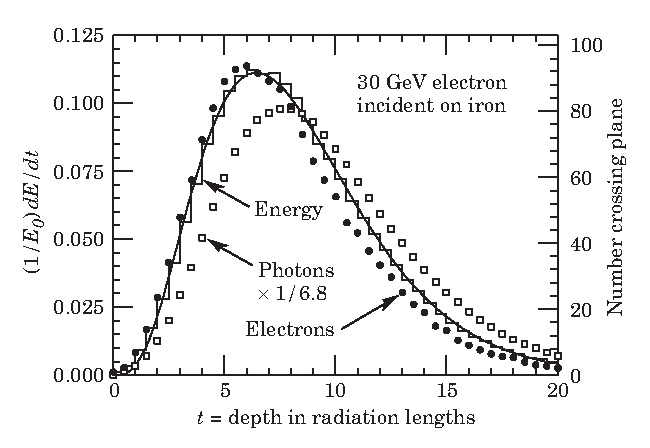
\includegraphics[width=0.65\textwidth]{photon/EMlong}}
\caption[Simulated longitudinal electromagnetic shower profile as a function of depth for electrons and photons.]
{An EGS4 simulation of a 30\,GeV electron-induced electromagnetic shower in iron. The histogram shows fractional energy deposition as a function of radiation lengths, and the curve is a gamma-function fit to the distribution. Circles and squares are the number of electrons and photons respectively with total energy greater than 1.5\,MeV crossing planes with scale on right. Plot is taken from \cite{Agashe:2014kda}.}
\label{fig:photonEMlongProfile}
\end{figure}

%The \RM of a material  describes the EM transverse  shower profile.
The EM transverse shower profile can be described as  a narrow cone widening as the shower develops. 90\% of the shower energy  is contained in a fiducial cylinder with a radius of one \RM, along the direction of the shower.

%%The dense shower core of the transverse profile allows the separation of two EM showers using a two-dimensional peak-finding algorithm, explained in a later section.



%Photon reconstruction is an important part of \pandora reconstruction. A good photon reconstruction should provide a good single photon completeness and purity, as well as a good photon separation resolution. For many physics processes, heavy particles decaying into photons, such as \Ptau lepton and \Ppizero. Photon reconstruction is crucial for reconstructing these heavy particles.

%The photon reconstruction presented in this chapter has improved the photon reconstruction completeness by reducing the fragments. The photon separation resolution has  also been improved. This work has been published in a conference proceeding \cite{Xu:2016rcz}. The improved  photon reconstruction has benefited many physics analyses involving photons. The most recent example is the  \HepProcess{\PHiggs \to \Pgamma \Pgamma} analysis at \rootS{3} at \CLIC \cite{Kacarevic:higgsToGammaGamma}.

%This set of photon related algorithms have been incorporated into the default reconstruction chain in \pandora. The \CLIC simulation studies have benefited from the improved photon reconstructions in various physics process, such as  \HepProcess{ \PHiggs \to \Pgamma \Pgamma}.

\begin{comment}
Since the discovery of a particle consistent with being the SM Higgs boson in LHC at 2012 \cite{Aad:2012tfa,Chatrchyan:2012ufa}, our understanding of Standard Model has improved greatly. Yet limited by the underlying QCD interaction from proton-anti-proton collision, one has great difficulty to measure the properties of the Higgs precisely. Next generation electron-positron linear collider could hopefully make precision measurements of the Higgs sector and the Top quark sector \cite{Abramowicz:2013tzc}.

The leading candidates for next generation electron-positron linear collider are the International Linear Collider (ILC) \cite{Brau:2007zza}, and the Compact Linear Collider (CLIC) \cite{Linssen:2012hp}. The ILC has developed two detector models, namely the International Large Detector (ILD) \cite{Abe:2010aa} and the Silicon Detector (SiD) \cite{Aihara:2010zz}. The CLIC has developed two slightly modified detector models based on ILD and SiD \cite{Linssen:2012hp}. One key common feature of these next generation electron-positron linear colliders is the high granular calorimeter, which provides a great spatial resolution at the cost of the energy resolution. Particle flow algorithms (PFA) benefit from the spatial resolution from calorimeters, together with tracking information, to provide excellent a jet energy resolution. PandoraPFA, the most complicated and the best performing one, provides a jet energy resolution of less than 3.5\%, which is required for W/Z separation \cite{Thomson:2009rp,Marshall:2013bda}.

\begin{figure}[tbph]
\centering
{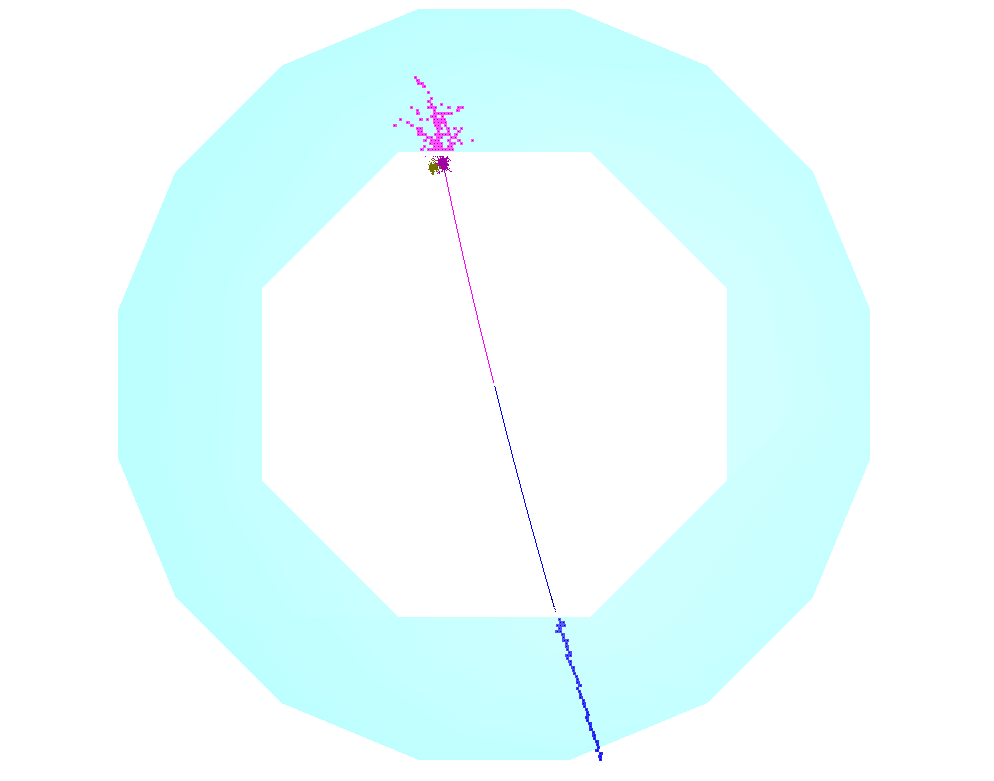
\includegraphics[width=0.5\textwidth]{images/tautauMod}}%

\caption{An event display of a simulated $\Pem\Pep\to \Ptauon\APtauon$ event. The blue region is the cross section of the Electromagnetic Calorimeter barrel region. The top $\Ptau$ decays into a charged $\Ppi$, two photons and neutrinos. The bottom $\Ptau$ decays into a muon and neutrinos.}
\label{fig:Tautau}
\end{figure}

Photon reconstruction is an important part of particle reconstruction. For many physics processes involving particles decaying into photons, such as $\Ptau$ lepton and $\Ppizero$, a good photon reconstruction, which provides a good single photon completeness and purity, as well as a good photon separation resolution, is crucial for reconstructing these particles.

\end{comment}

%\section{Electromagnetic shower}

\section{Overview of photon reconstruction in \pandora}

%\pandora is a multi-algorithm pattern-recognition software package for the event reconstruction and an implementation of the particle flow approach to calorimetry. A detailed discussion of the \pandora and the main steps of the \pandora event reconstruction can be found in \Section{sec:pandoraPandoraPFA}. The multi-algorithm approach of the \pandora allows each algorithm to deal with a particular issue in the reconstruction.


Five algorithms are developed to tackle different issues in the photon reconstruction. The most important photon algorithm is the \PhotonReconstruction algorithm. It reconstructs photons from calorimeter hits in the \ECAL, including forming a photon candidate and applying a photon ID test, with special treatments for photons close to charged particles. Three algorithms remove photon fragments at a later stage in the reconstruction. Two photon fragment removal algorithms remove fragments in the \ECAL, and one algorithm removes fragments in the \HCAL. The last photon algorithm is a photon splitting algorithm, which separates accidently merged photons. Samples used to produce figures in this chapter were reconstructed with the \ILD detector concept.
 %This algorithm is implemented at the early stage of the reconstruction.

%These algorithms improve the compsingle photon energy resolution.

%, which helps photon separation resolution.

%These algorithms together form the photon reconstruction in the \pandora. This chapter will first introduce the photon-induced electromagnetic shower in a calorimeter, followed by the description of each algorithm. The performance of the photon reconstruction will be provided in the last part of the chapter.

\begin{comment}
\pandora provides a framework for particle reconstruction \cite{Marshall:2015rfa}, as described in \Section{sec:pandoraPandoraPFA}. In the linear collider user case, it has a vast library of algorithms developed over years by many people. Each algorithm addresses one topological issue in the particle reconstruction. The essential part of the \pandora is track-cluster association  to find the best track-cluster pair, and re-clustering to find the best cluster consistent with the track. Other algorithms that identifies trackless clusters, such as muon clusters or photon clusters, would provide a cleaner environment for the track-cluster association, hence improving the jet energy resolution.

Photon identification in \pandora has two main mechanisms. The basic mechanism performs photon identification at the last step of the reconstruction  (see \Section{sec:pandoraPFOcreation}). The second more sophisticated photon identification is performed at an early stage of the reconstruction  (see \Section{sec:particleID}). The second algorithm identifies photon electromagnetic shower cores carefully in a dense jet environment. By removing photons from the environment, fewer calorimeters hits are left for charged particle reconstruction. Hence the overall reconstruction improves.

The \PhotonReconstruction algorithm in \pandora version 1 improves jet energy resolution by correctly identifying photon electromagnetic shower cores and leaving a cleaner environment for the track-cluster association. However, peripheral calorimeter hits to the shower cores may be reconstructed as separate particles (fragments). This lowers the reconstructed photon completeness and makes the number of reconstructed photons a less useful physical quantity. Also, the algorithm in \pandora version 1 leaves rooms for improvement of photon separation resolution.

This chapter presents a solution to photon reconstruction issues. The newly introduced algorithms reduces photon fragments and improves the photon separation resolution.

%Some part of the work has been published in a conference proceeding \cite{Xu:2016rcz}.

Firstly an overview of electromagnetic showers is presented. The \PhotonReconstruction algorithm will be described next, followed by fragment removal algorithms and photon splitting algorithms. This chapter will end with a discussion on performances of these photon related algorithms,  including comparisons with the previous photon algorithm.
%Algorithms related to photon reconstruction, fragmental removal and photon splitting, which are written or introduced by authors, will be discussed below.
\end{comment}

%The testing simulated data in this paper are generated either by WHIZARD \cite{whizard} or by the simple HepEvt generator. Events are simulated with GEANT4 \cite{Agostinelli:2002hh} in MOKKA \cite{MoradeFreitas:2002kj}. Jet fragmentation was performed with PYTHIA \cite{Sjostrand:1995iq} and the particle reconstruction was done by PandoraPFA \cite{Marshall:2015rfa} in MARLIN reconstruction framework \cite{Gaede:2006pj}, in ILD\_o1\_v6 detector model. The iLCSoft v17-01-07 was used. Different versions of PandoraPFA were used for the comparison purpose.




\section{\PhotonReconstruction algorithm}
\label{sec:photonRecostrcution}


The \PhotonReconstruction runs at an early stage of the reconstruction, before the charged particle reconstruction.   Main steps of the \PhotonReconstruction algorithm, shown in \Figure{fig:photonPhotonRecoFlow}, are:  forming photon clusters; finding photon candidates; photon ID test; and optional fragments removal.


%It corresponds to ``Particle ID'' stage in the \pandora reconstruction, described in \Section{sec:particleID}.
%Finding photon candidates uses the transverse EM shower profile information, which requires a  two dimensional peak finding algorithm, further explained in \Section{sec:peakFinding}. The photon ID test involves a multi dimensional likelihood classifier, which is described in \Section{sec:photonLikelihood}. The optional fragment removal algorithm shares a common code base case class with another photon fragment removal algorithm. Hence two photon fragment removal algorithms are discussed together in \Section{sec:photonFragRemoval}.

\begin{figure}[tbph]
\centering
{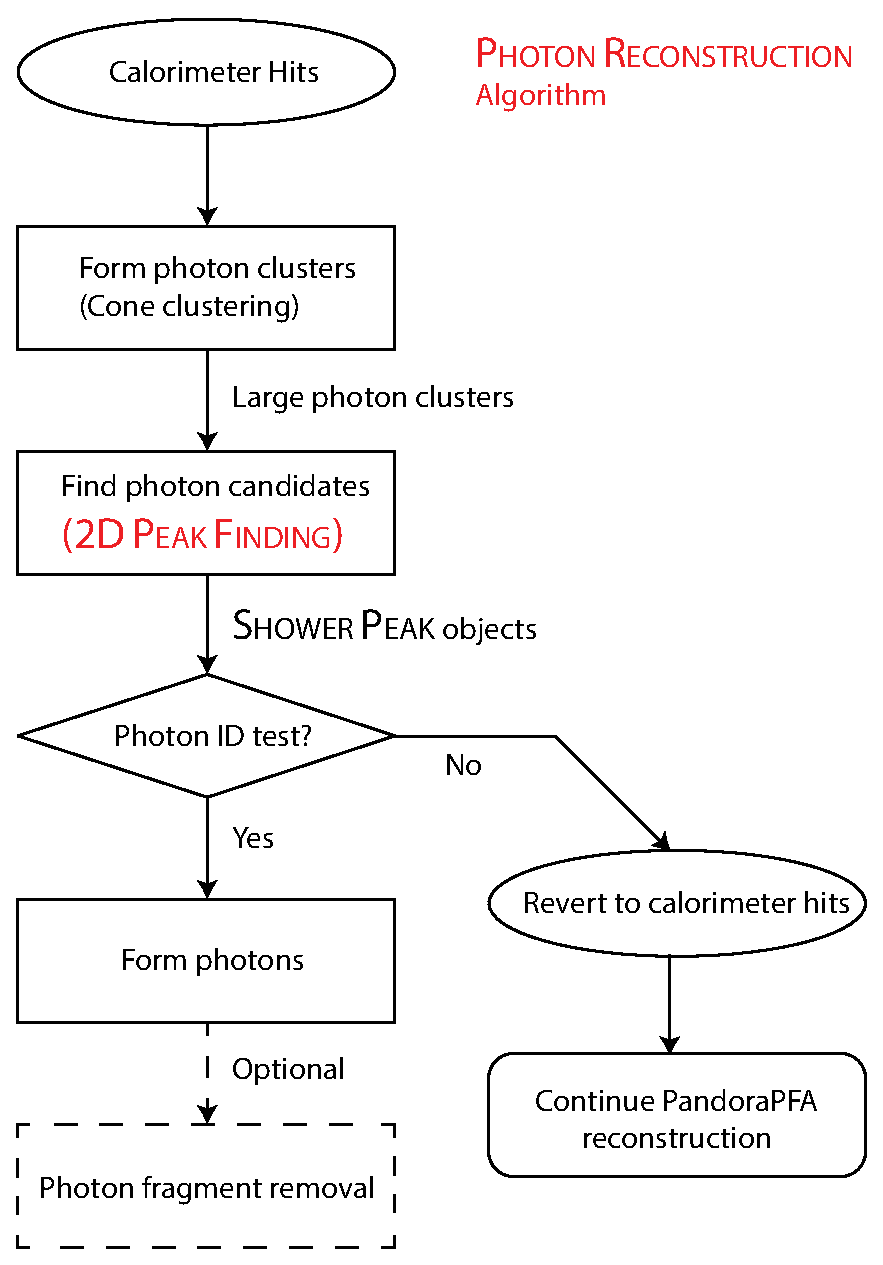
\includegraphics[width=0.65\textwidth]{photon/photonRecoFlow2}}
\caption[A flow diagram of the \PhotonReconstruction algorithm.]
{Main steps of the \PhotonReconstruction algorithm: forming photon clusters; finding photon candidates; photon ID test; and optional fragments removal.}
\label{fig:photonPhotonRecoFlow}
\end{figure}


\subsection{Forming photon clusters}

The inputs of the \PhotonReconstruction algorithm are calorimeter hits in the \ECAL that have not been used to form particles in previous algorithms. For example, muon reconstruction algorithms form muons and remove calorimeter hits associated with muons from the reconstruction. The  calorimeter hits associated with reconstructed muons are not used to form photons.

This step forms clusters from calorimeter hits in the \ECAL using the cone clustering algorithm. Since the target for reconstruction is the neutral photon, the cone clustering algorithm uses high-energy calorimeter hits in the \ECAL as initial seeds, instead of using track projections as initial seeds.  The clusters are formed in a way such that calorimeter hits from one photon would not be split into two clusters, but one cluster may contain calorimeter hits from  multiple photons.


%The algorithm uses  the cone clustering algorithm  provided inside \pandora to form clusters.   %The parameters for the cone clustering are such that  forming large clusters is preferred.

\subsection{Finding photon candidates}
\label{sec:photonCandiate}

This step refines photon clusters into smaller photon candidates. Each photon candidate should contain calorimeter hits from one photon only. If a cluster contains calorimeter hits from several photons, the three-dimensional cluster will be split into several smaller clusters (photon candidates).

The three-dimensional splitting problem is harder than a two-dimensional one. Therefore, a translation is needed to map the three-dimensional problem to a more manageable two-dimensional problem. This translation relies on the characteristic EM transverse shower profile. Along the direction of the shower, an EM shower can be modelled as a dense shower core with peripheral calorimeter hits around the core. When the energies of the calorimeter hits of the cluster are projected onto a two-dimensional plane, an EM shower core would appear as a mountain-like structure in the plane. \FIGURE{fig:photonPeakFinding} shows an example of a cluster projected onto a two-dimensional plane, where two EM showers are identified. Hence, by identifying a peak in the two-dimensional plane, the EM shower core is identified.

%the energy deposition projection of two photons candidates. U and V axis are two arbitrary orthogonal axis in the transverse plane perpendicular to the direction of photons. Z axis shows the sum of the calorimeter hit energy in GeV. The bin size corresponds to the square \ECAL cell size.


%To reduce the problem of splitting a three dimensional clusters (a collection of hits) into a manageable two dimensional problem.

%The large photon clusters are split into smaller photon candidates, using two-dimensional shower profiles. The candidates close to a track projection are deemed as non-photons. Identifying photon candidates within a large photon cluster relies on the characteristic electromagnetic showers, in particular the transverse distribution. A energetic photon or electron hits the absorber layers of the \ECAL, it initiates an electromagnetic shower, where electron pair production and bremsstrahlung produce more low-energy photons and electrons. The transverse distribution is characterised by a narrow cone, widening while the shower develops.

%To view the transverse shower distribution, a two-dimensional energy deposition projection is constructed in the plane perpendicular to the direction of the cluster. \Figure{fig:photonPeakFinding} shows the energy deposition projection of two photons candidates. U and V axis are two arbitrary orthogonal axis in the transverse plane perpendicular to the direction of photons. Z axis shows the sum of the calorimeter hit energy in GeV. The bin size corresponds to the square \ECAL cell size.

\begin{figure}[tbph]
\centering
{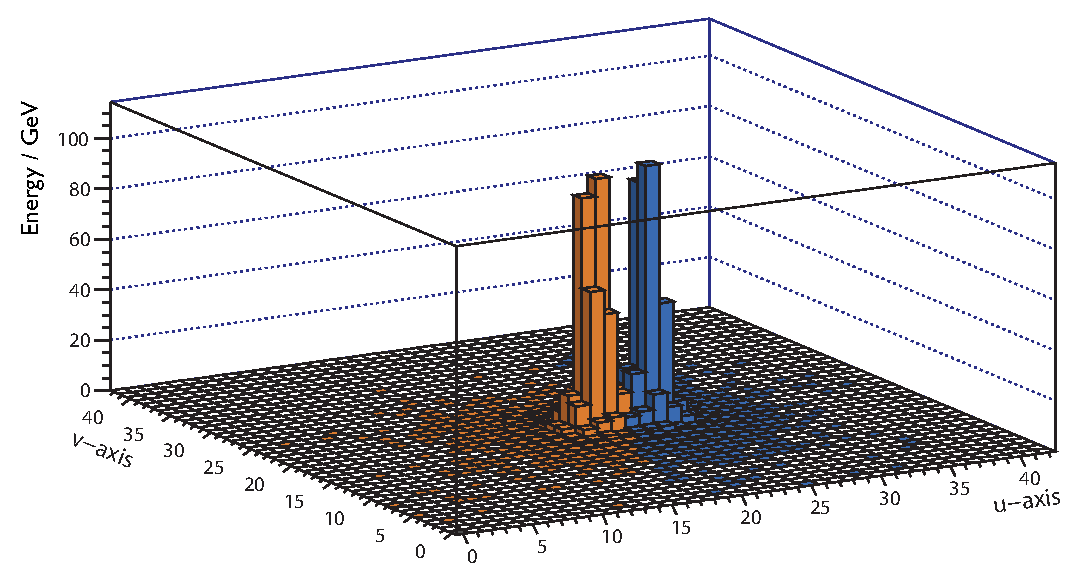
\includegraphics[width=0.85\textwidth]{photon/peakFindingMod}}
\caption[Example of projecting a large photon cluster containing two photons.]
{Two 500\,GeV photons (yellow and blue) within a  cluster, just resolved in a transverse plane orthogonal to the direction of the flight of the cluster.  The axes U and V are orthogonal axes in units of the \ECAL cell sizes. The height of a bin in the histogram is the sum of the calorimeter hit energy associated with the bin.}
\label{fig:photonPeakFinding}
\end{figure}

%obtained by projecting the energy deposition of the calorimeter hits of the cluster in the plane.

A high-performance two-dimensional peak-finding algorithm is the key to identify multiple photon candidates within a cluster. Due the complexity of the peak finding procedure, a peak-finding algorithm is developed and discussed in \Section{sec:peakFinding}. The output of the two-dimensional peak-finding algorithm is a collection of \ShowerPeak objects. Each \ShowerPeak object corresponds to one photon candidate and associated calorimeter hits.

\subsection{Photon ID test}
\label{sec:photonIDtest}

This step applies the photon ID test on the \ShowerPeak object. The photon ID test uses  a multidimensional likelihood classifier. A set of variables, which exploit features of electromagnetic showers, are used. The response from the classifier determines if a \ShowerPeak object is a photon. If it passes the photon ID test, the \ShowerPeak object would be tagged as a photon and the photon is not used in the subsequent event reconstruction. If a \ShowerPeak object   fails the  photon ID test, the \ShowerPeak object  will be discarded. Calorimeter hits associated with the discarded  \ShowerPeak object will be passed onto the next stage of the reconstruction. The likelihood classifier used in the photon ID test is further discussed in \Section{sec:photonLikelihood}.

%The identified photon re-enters the event reconstruction at the fragment removal stage.

\subsection{Photon Fragment removal}
\label{sec:photonRecoFragRemoval}

The  photon fragment removal algorithm merges small photon fragments to identified photons. The algorithm is optional as it is not used by the default setting of the event reconstruction. Since this algorithm shares the same logic as another fragment removal algorithm, two algorithms are discussed togethers in \Section{sec:photonFragRemoval}.

%only differing in the cut-off values for merging metrics, this step be discussed in \Section{}.

This step marks the end of the \PhotonReconstruction algorithm. The outputs are reconstructed photons, separated from calorimeter hits that are not associated with photon.
%The candidate passed the test will be kept in a separate container for photons only

\section{\peakFinding algorithm}
\label{sec:peakFinding}

As discussed in \Section{sec:photonCandiate}, identifying photon candidates inside a cluster is translated into identifying peaks in a two-dimensional plane, using a two-dimensional peak-finding algorithm (\peakFinding algorithm). The \peakFinding algorithm aims to correctly identify peak positions in a two-dimensional histogram and to associate non-peak bins to identified peaks.

% An example of two photons resolved in a two dimensional plane is shown in the \Figure{fig:photonPeakFinding}.
%  calorimeter hits of

There are two variants of the \peakFinding algorithm: the neutral cluster variant and the charged cluster variant. Main steps of the neutral cluster variant are shown in \Figure{fig:photonPeakFindingFlowNeutral}: initialising a two-dimensional histogram; projecting  calorimeter hits to the histogram; identifying local peaks; associating non-peak bins to peaks; filtering peaks; and forming \ShowerPeak objects.

%Since charged hadrons would deposit tracks in the tracking system, extra care is taken when a cluster is close to the projection of the track in the front of the \ECAL.
%The base algorithm is  the neutral cluster variant. The charged cluster variant is only used when the cluster is close to the projection of a track onto the front of the \ECAL. 
% The neutral cluster variant is described first, followed by description of the modification of the algorithm to treat clusters close to track projections.

\begin{figure}[tbph]
\centering
{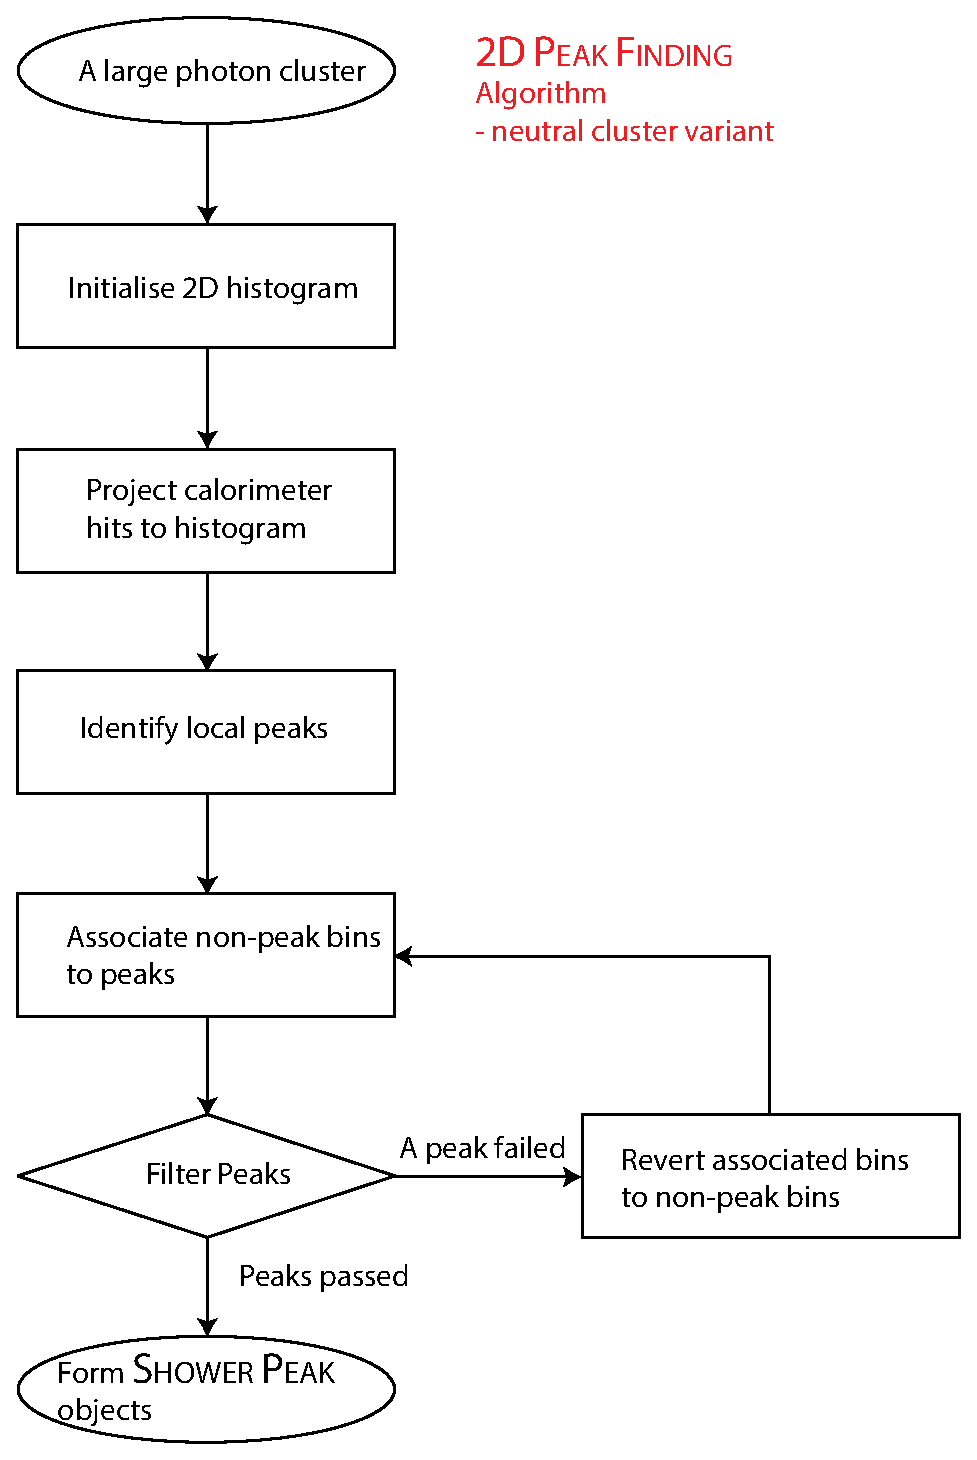
\includegraphics[width=0.7\textwidth]{photon/2DpeakFinding2}}
\caption[Flow chart for \peakFinding algorithm neutral cluster variant.]
{Main steps of the  neutral cluster variant of the \peakFinding algorithm: initialising a two-dimensional histogram; projecting  calorimeter hits to the histogram; identifying local peaks; associating non-peak bins to peaks; filtering peaks; and forming \ShowerPeak objects.}
\label{fig:photonPeakFindingFlowNeutral}
\end{figure}

\subsection{Initialising  two-dimensional histogram}

This step initialises a two-dimensional (2D) histogram to host the projection of the calorimeter hits of the cluster. For the best resolving power between EM showers, the projection direction is chosen to be the direction of the cluster. Two axes of the two-dimensional histogram are chosen such that the axes and the direction of the cluster form an orthogonal basis  in the three-dimensional space.

%The axes are labelled as  U and V axis in \Figure{fig:photonPeakFinding}.



\subsection{Projecting calorimeter hits to histogram}

%For a finite-sized 2D histogram, t
This step projects the calorimeter hits associated with the cluster onto the 2D histogram. The projection is chosen such that the cluster centroid position is projected onto the centre of the histogram. The distance between the calorimeter hit position and the cluster centroid position is then converted into a distance vector to be used to project the calorimeter hit. The distance vector, $\vec{s_{i}}$, of a calorimeter hit $i$, is defined as:
\begin{equation}
\vec{s_{i}} = \frac{\vec{a_{i}} -  \vec{\angles{a}}}{d_{cell}},
\end{equation}
where $\vec{a}$ is the three-dimensional position of the calorimeter hit $i$;  $\vec{\angles{a}}$ is the centroid position of cluster $a$; and $d_{cell}$ is the  \ECAL square cell length. The coordinate of the calorimeter hit projection onto the histogram is calculated from the scalar products of the distance vector ($\vec{s_{i}}$) with the axes vectors.
% One bin size along either axes on the 2D histogram corresponds to one \ECAL square cell length.

The height of a bin in the 2D histogram is the sum of the energies associated with the calorimeter hits that fall in that particular bin. Each bin contains calorimeter hits that projected onto the bin. One bin size along either axes on the 2D histogram corresponds to one \ECAL square cell length.

%The issue with the histogram size being finite is discussed in \Section{sec:photonPeakFindingInclusive}.

\subsection{Identifying local peaks}

This step identifies all local peaks in the 2D histogram. A local peak is defined as a bin where its height is above all eight neighbouring bins. All bins in the 2D histogram are  iterated to identify all local peaks. \FIGURE{fig:photonPeakFindingPeakOnly} shows an example of a 2D histogram with two local peak bins (orange and blue) identified. Red bins are non-peak bins.

%Hence the processing time is $O\left(N^2\right)$, where $N$ is number of bins in one axis.
%For example, in \Figure{fig:photonPeakFinding}, there are clearly two peaks, both colour coded.



\begin{figure}[tbph]
\centering
{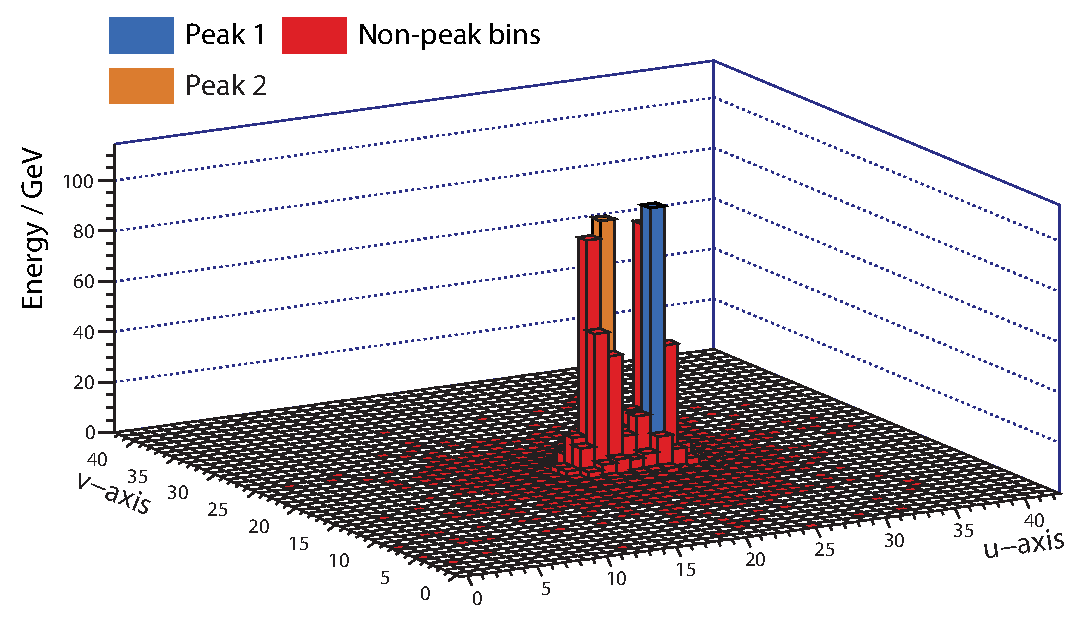
\includegraphics[width=0.85\textwidth]{photon/peakFindingPeakOnly}}
\caption[Example of projecting a large photon cluster containing two photons.]
{Two peak bins, orange and blue, are identified. Red bins are non-peak bins.}
\label{fig:photonPeakFindingPeakOnly}
\end{figure}


\subsection{Associating non-peak bins to peaks}

Having identified all local peaks, this step associates non-peak bins to a particular peak based on the energy of the peak and the distance of the non-peak bin to the peak bin. A non-peak bin should be associated to a high-energy peak bin that is close to the non-peak bin.

%The energy dependence is needed as the transverse EM shower width increases with the increase of the energy of the EM shower. The distance dependence is needed because the EM showers have dense shower cores, and
%To associate non-peak bins to the correct peak bin, the peak bin is
%The peak bin to associate a non-peak bin is chosen by minimising the metric:
A non-peak bin is associated with the peak bin that gives the smallest value of the metric:
\begin{equation}
\frac{d_{i}}{\sqrt{E_{i}}}
\end{equation}
where $d_{i}$ is the Euclidean distance between a non-peak bin and a  peak bin $i$ on the 2D histogram, and $E_{i}$ is the height (energy) of the peak bin $i$. For each non-peak bin, the metric is iterated over all peak bins to find the peak bin that produces the smallest metric. In the example of the 2D histogram in \Figure{fig:photonPeakFindingPeakOnly} with two peaks identified, the result after associating non-peak bins to peak bins is shown in \Figure{fig:photonPeakFinding}.

%Alternative metrics provided in the algorithm include $d_{i}$, $\frac{d_{i}}{{E_{i}}}$, and $\frac{d_{i}}{{E_{i}^2}}$. The default metric is chosen due to a good balance between distance and energy of the peak.

%And EM shower is typically narrow transversely.

\subsection{Filtering peaks}

The performance of the \peakFinding algorithm is improved by peak filtering. In a 2D histogram, such as the one in \Figure{fig:photonPeakFinding}, major peaks with many associated non-peak bins correspond most likely  to physical photons, while minor peaks with a few associated non-peak bins are more likely from fluctuations in the energy deposition of the EM shower. To select only major peaks and to discard minor peaks, every time after all non-peak bins are associated with peak bins, peaks with fewer than three bins associated (including the peak bin) are discarded. These discarded bins are re-associated with other peak bins. This  process iterates until all peak bins have at least three bins associated.

%The peak filtering step also allows bins with heights below a critical value to not participate in the peak finding. The default value is set such that only non-empty bins are used.

After  filtering peaks,  \ShowerPeak  objects are created . One \ShowerPeak object contains one peak bin and associated non-peak bins. The associated calorimeter hits within the bins are attached to the \ShowerPeak object as well. If multiple peaks are identified in a cluster, multiple \ShowerPeak objects are created as outputs.

%This marks the end of the neutral clusters variant of the \PhotonReconstruction algorithm, outlined in \Figure{fig:photonPeakFindingFlowNeutral}.

%The  \ShowerPeak object is also referred to as the photon candidate.

\subsection{\peakFinding algorithm charged cluster variant}
\label{sec:photon2Dtrack}

In a dense jet environment, if a photon next to a charged hadron is carefully reconstructed, the charged particle reconstruction is improved.

%If  a photon candidate is close to the projection of the track onto the front of the \ECAL, it is more likely that the candidate is a charged hadron. Misidentifying a charged hadron as a photon leads to a significant degradation in the reconstruction performance, because there will be double counting of energies from the track and from the charged hadron misidentified as a photon. However,


This step aims to carefully identify photon candidates next to charged hadrons, by using track information and features of EM showers. An EM shower typically starts in the first few layers of the \ECAL with  direction of the EM shower largely unchanged when the shower develops.


\FIGURE{fig:photonPeakFindingFlow} shows the main steps in the full \peakFinding algorithm, including the treatment of clusters close to tracks. The first step of the algorithm, "Close to track", determines if a cluster is close to a track. If the distance between a cluster and the closest track projection onto the front of the \ECAL is fewer than 3\,mm, the charged cluster variant of the \peakFinding algorithm is applied to the cluster.

\begin{figure}[tbph]
\centering
{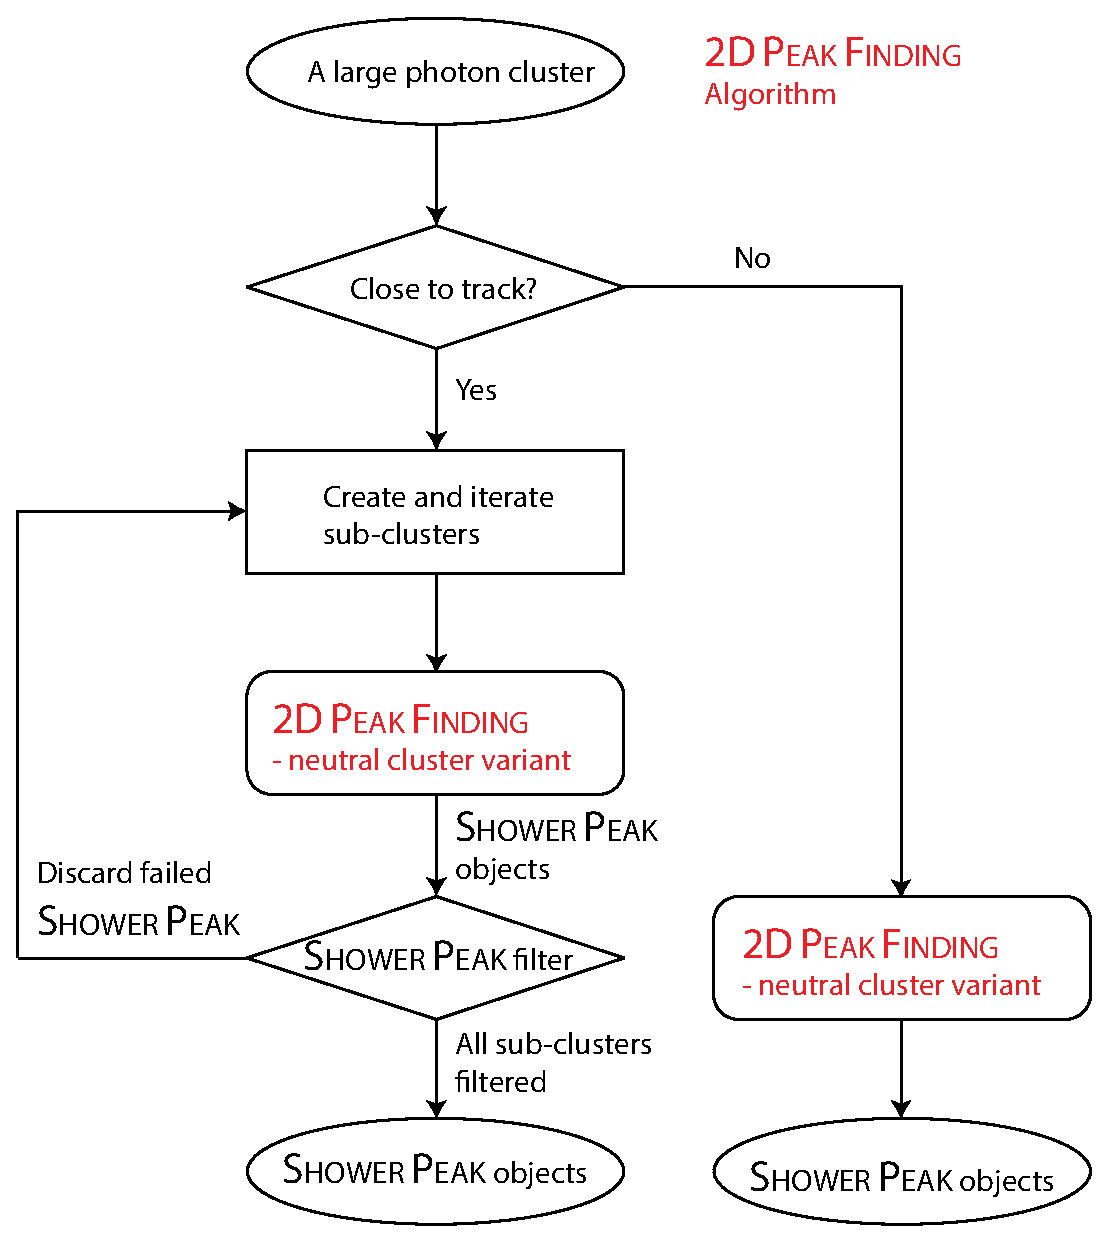
\includegraphics[width=0.8\textwidth]{photon/2DpeakFindingTrack}}
\caption[Flow chart for \peakFinding algorithm.]
{Main steps of the  \peakFinding algorithm, including the charged cluster variant: identifying whether the cluster is close to a track; creating and iterating over sub-clusters; applying \peakFinding algorithm neutral cluster variant to sub-clusters; filtering \ShowerPeak objects in sub-clusters; creating final \ShowerPeak objects.}
\label{fig:photonPeakFindingFlow}
\end{figure}


The "Create and iterate over sub-clusters" step performs the following. The \ECAL is sliced longitudinally to create fiducial volumes. For example, the default three slices will result in three \ECAL fiducial volumes. Each fiducial volume covers the  space from the front of the \ECAL to a third, to two thirds, and to the back of the \ECAL. Three sub-clusters are created from calorimeter hits of the cluster that are contained in each fiducial volume.

After creating sub-clusters, the neutral cluster variant of the  \peakFinding algorithm is applied to each sub-cluster to find peaks.  The sub-cluster in the first a third of the \ECAL is processed first. The sub-cluster in the whole of the \ECAL is processed last. For each sub-cluster,  \ShowerPeak objects are created from the  \peakFinding algorithm.

The \ShowerPeak objects created from each sub-cluster undergo the "\ShowerPeak filter" step. The order of the \ShowerPeak objects to filter peaks is the same order of creating the sub-clusters. All peaks from the first sub-cluster are preserved. For the next sub-cluster, a peak  is only preserved if the peak bin position is the same as a peak bin position in the previous sub-cluster, allowing a shift in the peak bin position by no more than one neighbouring bin. Furthermore, if a peak bin is within one neighbouring bin of a track projection bin, the peak is discarded. Only the peaks in the last sub-cluster that are not discarded will be used to form the final \ShowerPeak objects. The track projection bin in the 2D histogram is the bin where the track position, which is projected position onto the front of the \ECAL, projects onto the 2D histogram.

% position of the track projection onto the front of the \ECAL projects onto the 2D histogram.

% preserved in every sub-cluster through the iteration of "\ShowerPeak filter" step

%The track projection bin is obtained by projecting the position to the 2D histogram.
% of the track projection onto the front of the \ECAL
%The non-preserved peak and the associated \ShowerPeak object are discarded.
%, reconstructed using the \ILD detector model

\FIGURE{fig:photon2DpeakCharge} illustrates an example of three sub-clusters created during the charged variant of the \peakFinding algorithm. Peaks with associated bins and track projection bins are labelled. \FIGURE{fig:photon2DpeakCharge1} shows the first sub-cluster, created with calorimeter hits of the cluster in the first 10 layers of the \ECAL. One peak is identified. \FIGURE{fig:photon2DpeakCharge2} shows the second sub-cluster, created with calorimeter hits of the cluster in the first 20 layers of the \ECAL. The one peak in the second sub-cluster is in the same position of the peak in the first sub-cluster. Hence, the peak in the second cluster is preserved. \FIGURE{fig:photon2DpeakCharge3} shows the third sub-cluster, created with calorimeter hits of the cluster in the \ECAL. Three peaks are identified. However, only one peak (blue) shares the  same position of the peak in the second sub-cluster. Hence, only that peak (blue) is preserved. The preserved peak and associated bins in the third sub-cluster are then used to create one \ShowerPeak object.


\begin{figure}[tbph]
\centering
  \begin{subfigure}[b]{0.65\textwidth}
    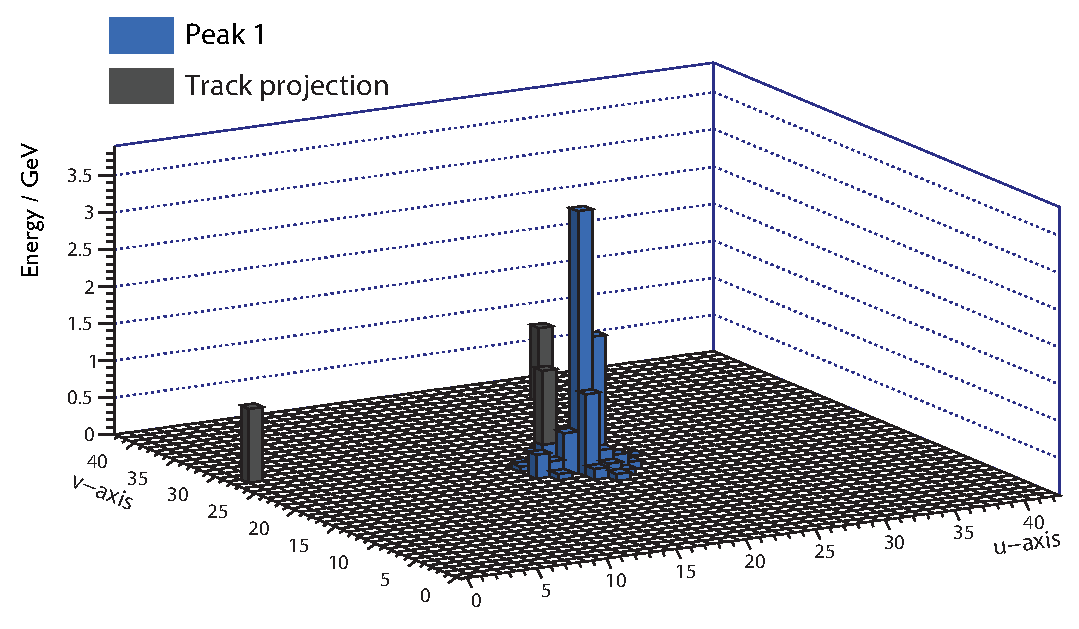
\includegraphics[width=\textwidth]{photon/2Dpeak/charge1}
    \caption{}
    \label{fig:photon2DpeakCharge1}
  \end{subfigure}
  \begin{subfigure}[b]{0.65\textwidth}
    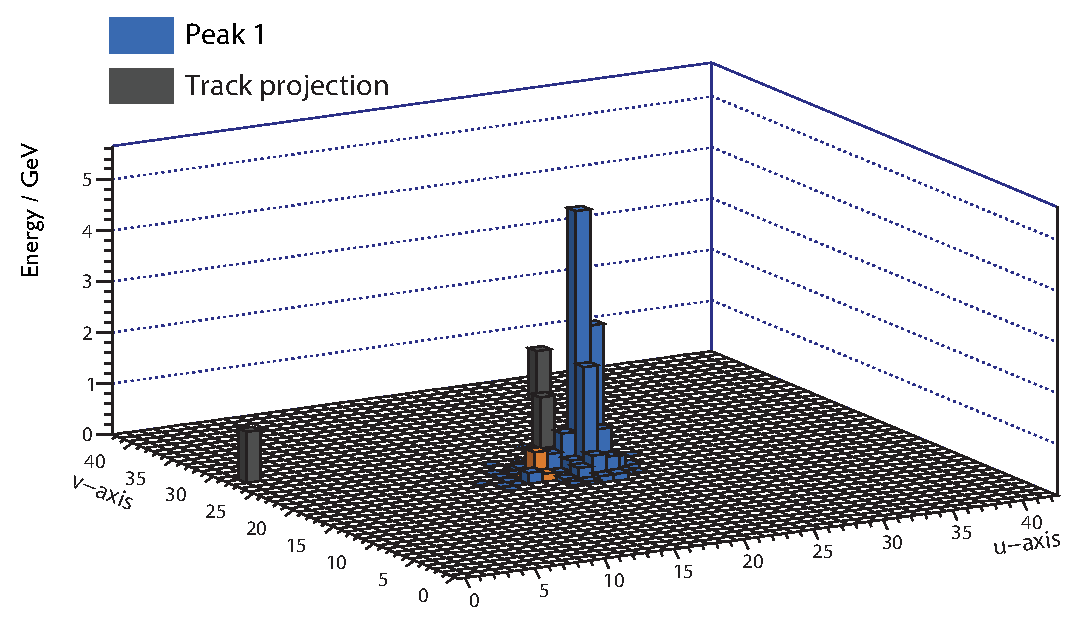
\includegraphics[width=\textwidth]{photon/2Dpeak/charge2}
    \caption{}
    \label{fig:photon2DpeakCharge2}
  \end{subfigure}
  \begin{subfigure}[b]{0.65\textwidth}
    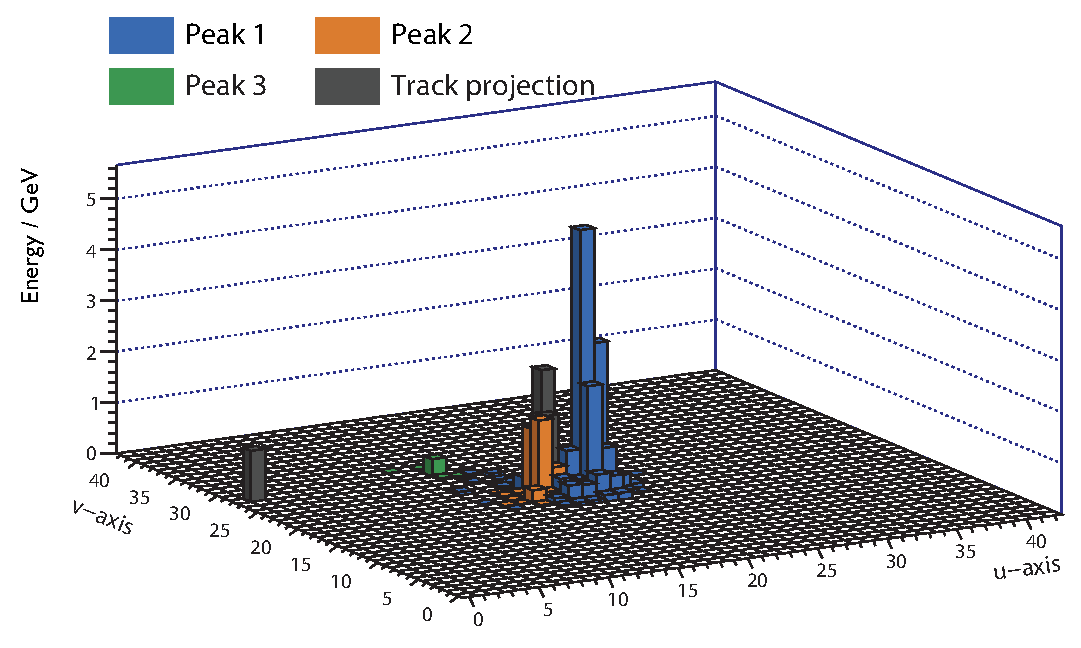
\includegraphics[width=\textwidth]{photon/2Dpeak/charge3}
    \caption{}
    \label{fig:photon2DpeakCharge3}
  \end{subfigure}
\caption
{An illustration of three sub-clusters created during the charged cluster variant of the \peakFinding algorithm. Peaks with associated bins and track projection bins are labelled.}
\label{fig:photon2DpeakCharge}
\end{figure}


\subsection{Inclusive mode}
\label{sec:photonPeakFindingInclusive}

%The 2D histogram is iterated many times during the algorithm.

The time complexity of iterating the 2D histogram is $O(n^2)$ for a $n$ bins by  $n$ bins sized histogram (default $n = 41$). Therefore, for the purpose of speed, it is undesirable to have  a large number of bins. Having a small finite-sized histogram speeds up the computation. However, because of the finite size of the histogram, only  calorimeter hits  projected onto the histogram would be considered by the peak finding algorithm. Calorimeter hits projected outside the histogram would not be used when \ShowerPeak objects are constructed. This behaviour is suitable if the algorithm is only interested in finding the EM shower cores, for example, the \PhotonReconstruction algorithm. However, for the purpose of photon splitting, all calorimeter hits from the parent photon should be used to form daughter photons. Hence the inclusive mode of the \peakFinding algorithm is developed, and allows calorimeter hits projected outside the histogram to be associated with identified peaks.


\section{Likelihood classifier for photon ID test}
\label{sec:photonLikelihood}

In \Section{sec:photonIDtest}, the photon ID test in the photon reconstruction algorithm is outlined. This section describes the multidimensional likelihood classifier used in the photon ID test in details.
%For each photon candidate, a set of variables are calculated and used to as inputs to the classifier.

%\subsection{Overview of Projective Likelihood}
%\label{sec:photonPDE}

\subsection{Variables used in likelihood classifier }

Variables used in the likelihood classifier exploit the differences between a characteristic electromagnetic shower and a hadronic shower, and the fact that a photon is less likely to be close to track projections onto the front of the \ECAL, than a cluster of a charged particle. Variables used in the classifier are listed in \Table{tab:photonPhotonIDvar}.

Two variables are obtained from the EM longitudinal shower profile: the variable $t_0$ is the start layer from the longitudinal shower profile, shown in \Figure{fig:photonLongProfileStart}; and $\delta{l}$ is fractional difference of the observed EM shower profile to the expected EM shower profile described in \Equation{eq:photonEMshower}:
\begin{equation}
\delta l = \frac{1}{E_0}\sum_{i}^{}\absOf{\Delta E_{obs}^i - \Delta E_{EM}^i },
\end{equation}
where $E_0$ is the energy of the EM shower; $\Delta E_{EM}^i$ is the energy of the expected EM shower profile in bin $i$;  $\Delta E_{obs}^i$ is the energy of the observed EM shower profile in bin $i$; the index $i$ is summed over the \ECAL layers as the EM shower is binned according to the \ECAL layers; and the quantity $\delta l$ is minimised as a function of the $t_0$. The $\delta l$ distributions for photons and non-photons are shown in \Figure{fig:photonLongProfileDiscrepancy}. For a true photon, $t_0$  and $\delta l $ are expected to be small, as an EM shower should start in the first few layers of the \ECAL and the observed EM shower profile should be similar to an expected EM shower profile.

Three variables are obtained from the transverse EM shower profile: the variable $\langle{w}\rangle$ is the energy weighted \rms distance of all bins in a \ShowerPeak to its peak bin, a measure of the transverse shower size, shown in \Figure{fig:photonPeakRms}; the variable $\delta{\langle{w_{UV}}\rangle}$ is the smallest ratio of the two energy weighted \rms distances of all bins in a \ShowerPeak to its peak bin in each of the U, V axis direction, a measure of the circularity of the transverse shower; the last variable, $\delta E_{cluster}$, is the  ratio of the energy of the \ShowerPeak object to the cluster energy, a measure of the dominance of the \ShowerPeak in a cluster.

The last variable used in the classifier, $d$, is the distance between the candidate and the closest track projection onto the front of the \ECAL. The \ShowerPeak object is less likely to be a photon if it is close to a track. The distributions of $d$ for photons and non-photons are shown in \Figure{fig:photonMinDistanceToTrack}.


\begin{table}[htbp] \centering \smallskip
\begin{tabular}{l r }
\hline
\hline
Categories&  Variables\\
\hline
EM longitudinal  shower profile & $\delta{l}$, $t_0$ \\
EM transverse  shower profile & $\langle{w}\rangle$, $\delta{\langle{w_{UV}}\rangle}$, $\delta E_{cluster}$ \\
Distance to track &  $d$ \\
\hline
\hline
\end{tabular}
\caption
{Variables used in the likelihood classifier for photon ID test.}
\label{tab:photonPhotonIDvar}
\end{table}

\begin{figure}[tbph]
\centering
  \begin{subfigure}[b]{0.45\textwidth}
    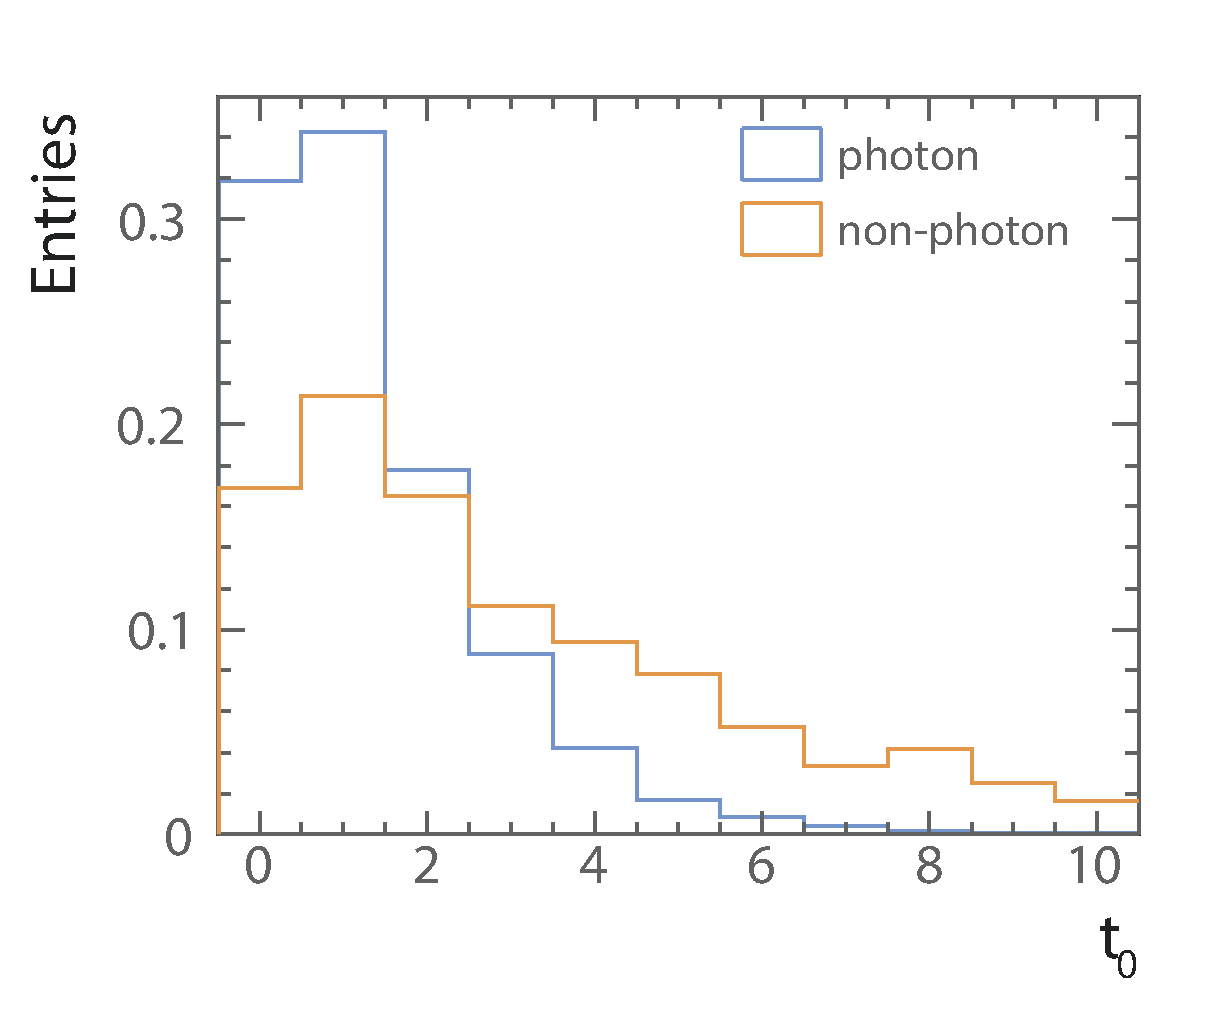
\includegraphics[width=\textwidth]{photon/likelihood/LongProfileStart2}
    \caption{}
    \label{fig:photonLongProfileStart}
  \end{subfigure}
  \begin{subfigure}[b]{0.45\textwidth}
    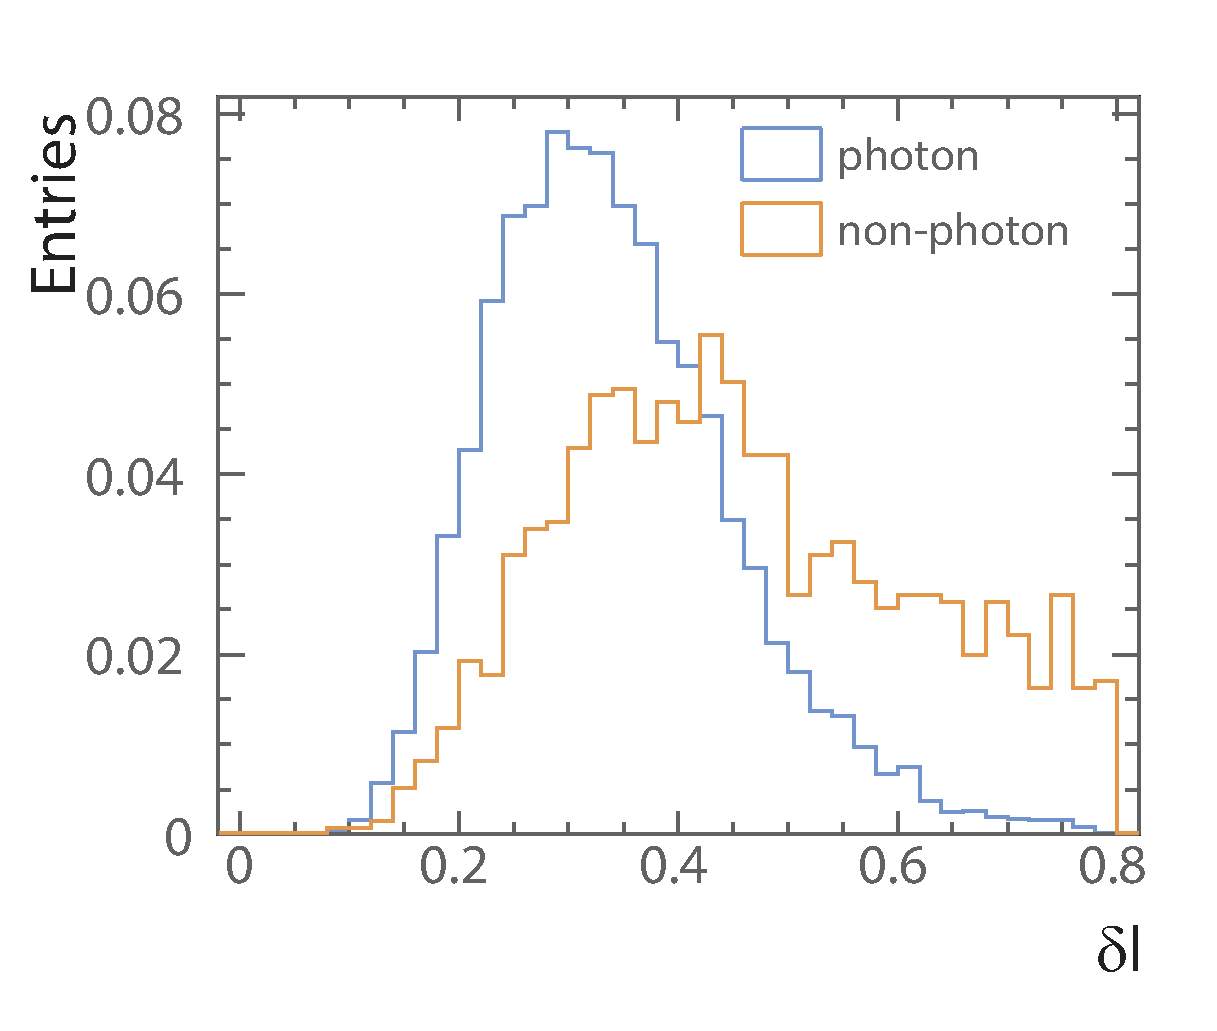
\includegraphics[width=\textwidth]{photon/likelihood/LongProfileDiscrepancy2}
    \caption{}
    \label{fig:photonLongProfileDiscrepancy}
  \end{subfigure}
  \begin{subfigure}[b]{0.45\textwidth}
    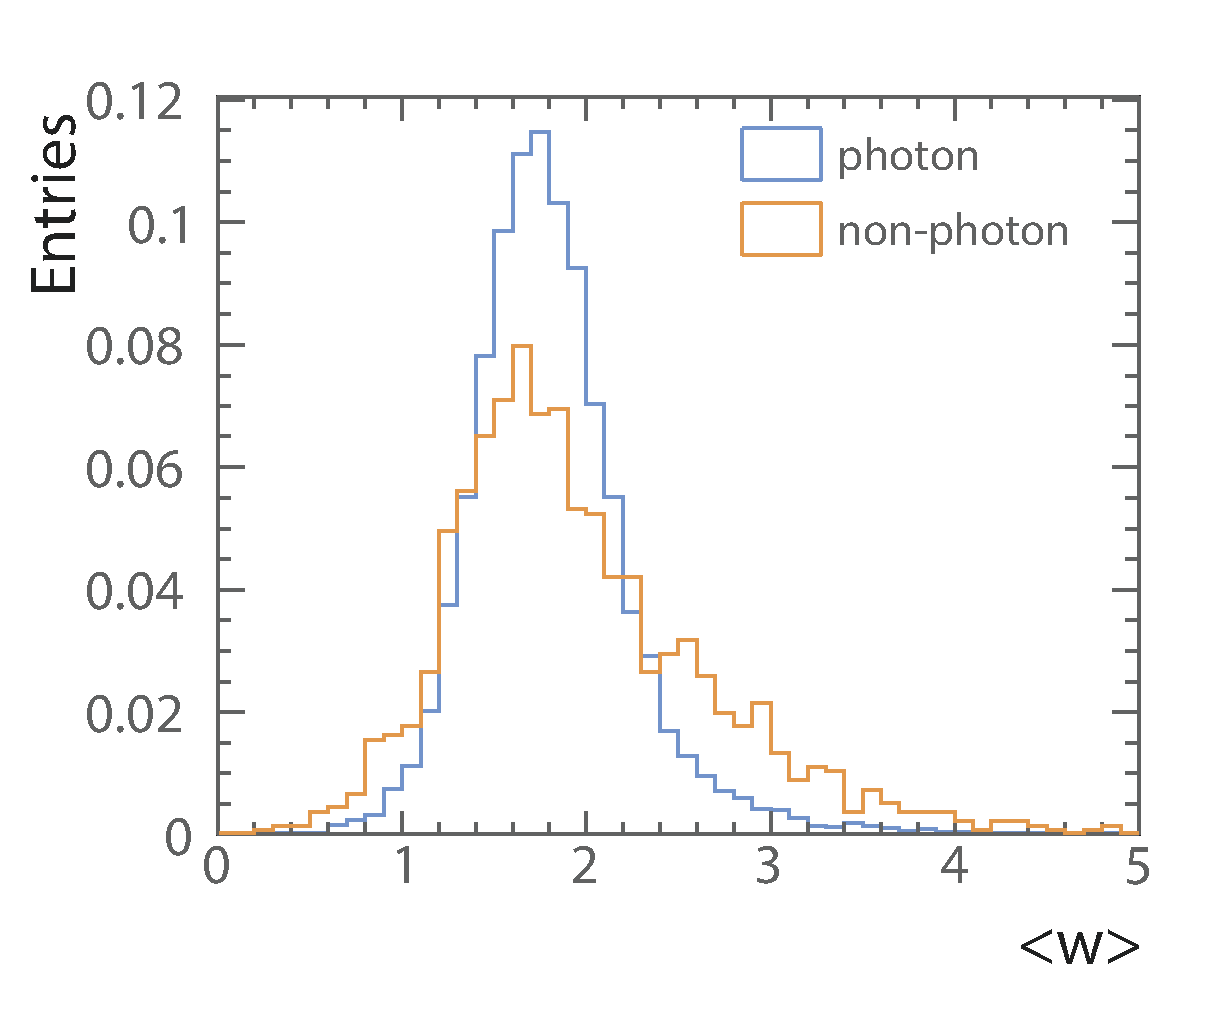
\includegraphics[width=\textwidth]{photon/likelihood/PeakRms2}
    \caption{}
    \label{fig:photonPeakRms}
  \end{subfigure}
  \begin{subfigure}[b]{0.45\textwidth}
    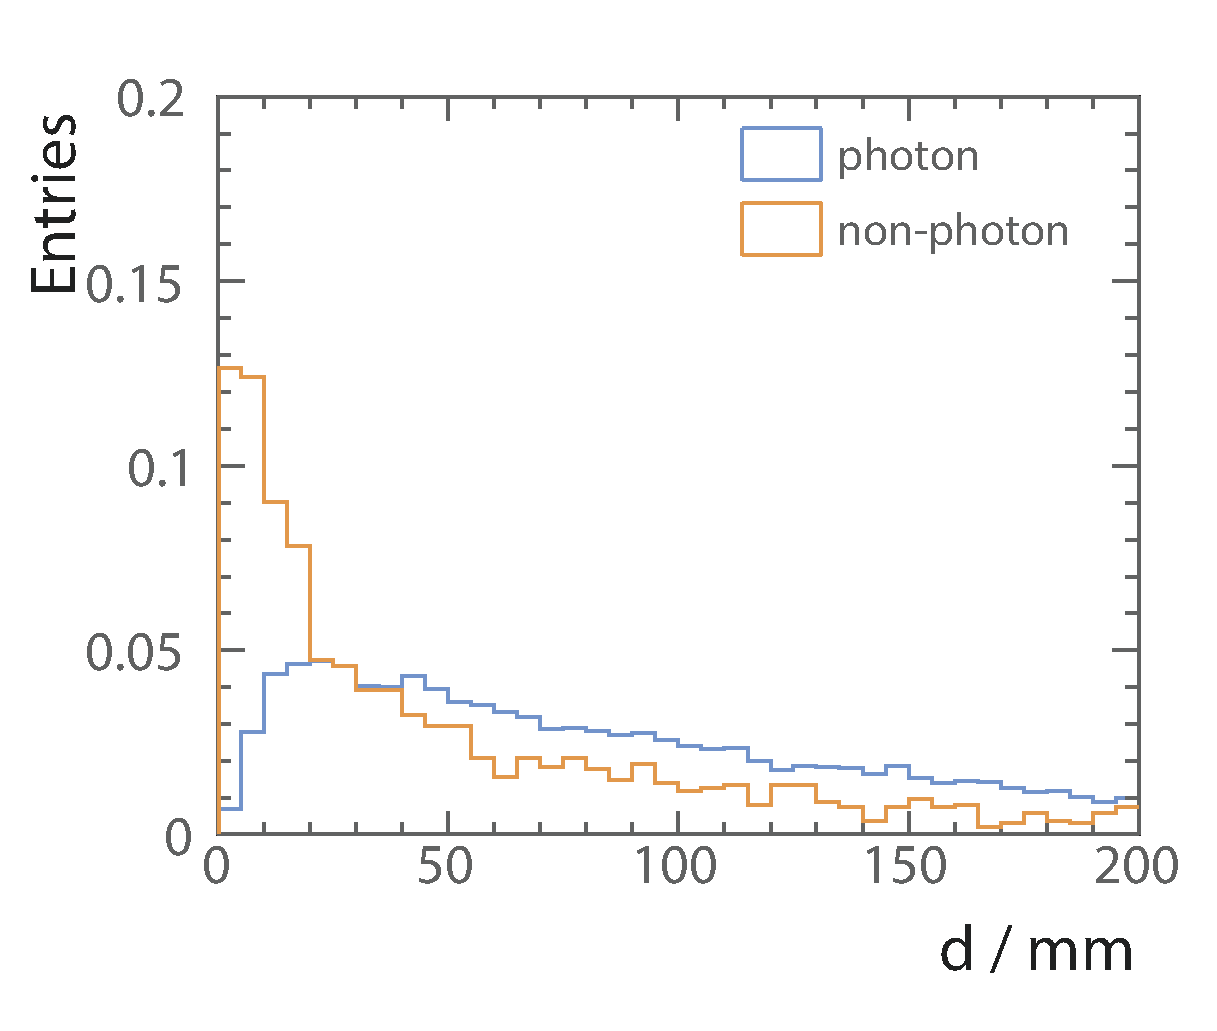
\includegraphics[width=\textwidth]{photon/likelihood/MinDistanceToTrack2}
    \caption{}
    \label{fig:photonMinDistanceToTrack}
  \end{subfigure}
\caption
{Distributions for a) the start layer from the longitudinal shower profile ($t_0$), b)  the fractional difference of the observed shower profile to the expected EM shower profile ($\delta{l}$), c) the energy weighted \rms distance of all bins in a \ShowerPeak to its peak bin ($\langle{w}\rangle$), and d) the distance between the photon candidate and the closest track projection onto the front of the \ECAL ($d$). The area under each curve is normalised to unity. The particle ID is determined using the truth information. All plots are produced with  simulated \eeZuds, at \rootSGeV{500}.}
\label{fig:photonVarLikelihood}
\end{figure}



%  Candidate with energy below 0.2\,GeV would not be examined in this step, as there are far more non-photons than photons and the classifier makes mor.

\subsection{Projective Likelihood classifier}


Projective likelihood classifier  with probability density estimators is used  for the photon ID test due to its  low requirement on computing resources, comparing to a boost decision tree classifier or a neutral network classifier.

The probability distributions of each variable for photons and non-photon particles are obtained in the training stage. The distributions of these variables are normalised to probability distribution, stored in binned histograms. The classifier is improved by realising the variable distributions varies with photon energies. Thus the variables distributions are stored separately for different photon energy ranges. There are 8 photon energy ranges, obtained by binning the distribution of photon energies at 0.2, 0.5, 1, 1.5, 2.5, 5, 10, 20\,GeV. The variable distributions for non-photon particles are binned in the same energy ranges, according to the energy of the non-photon.

The training stage of the classifier uses simulated  \eeZuds, at a centre-of-mass energy of 500\,GeV. The events at the centre-of-mass energy of 500\,GeV allow the training of photon with energies greater than 20\,GeV.

%Thus these distributions are divided by a range of photon energies. The default energy bins edges are

In the applying stage of the classifier, for a given candidate with the candidate energy in the  energy bin $\alpha$, the classifier output is given by
\begin{equation}
\uprightMath{PID_\alpha} = \frac{N \prod_{i}^6{P_{i}}}{N \prod_{i}^6{P_{i}} + N' \prod_{i}^6{P'_{i}}}
\end{equation}
where $P_{i}$ and $P'_{i}$ are the values of the bins that the candidate fallen in the $i^{th}$ variable probability distributions  of the  respective photon and non-photon particles in the energy bin $\alpha$; the variables $N$ and $N'$ are the number of respective photons and non-photon particles in the energy bin $\alpha$ in the training sample.


During applying stage of the classifier, a candidate passes the photon ID test if
\begin{equation}
\begin{cases}
  \text{PID} > 0.6, & \text{if}\ 0.2 < E < 0.5\,\text{GeV}\\
  \text{PID} > 0.4, & \text{if}\ E \geqslant 0.5\,\text{GeV}
\end{cases}
\end{equation}
where $E$ is the candidate energy. Two values of the cuts on $\text{PID}$ is because that it is more likely to misidentify a low-energy particle as a photon. A low-energy EM shower does not have a dense shower core, and is more difficult to identify. Hence for candidates with energies between 0.2 and 0.5\,GeV, \uprightMath{PID > 0.6} is required instead of \uprightMath{PID > 0.4}.

%An EM shower from a high-energy photon is more distinct than the hadronic shower from a non-photon of the same energy, than the difference between a low-energy  EM shower and hadronic shower.

%reflect the different confidence levels of the photon ID test with different candidate energies.

%The test is more cautious with low-energy candidates.


\section{Photon fragment removal algorithm in the \ECAL}
\label{sec:photonFragRemoval}
During the reconstruction, it is possible that a core of the photon electromagnetic shower is identified as a photon (the main photon), but the outer part of the shower is reconstructed as a separate particle (the fragment), and identified as a photon or a neural hadron. \FIGURE{fig:photonEvtDspPhotonFrag} shows a typical creation of such a photon fragment, reconstructed with \pandora version 1. A fragment typically does not have the electromagnetic shower structure, and has a much lower energy than a main photon.

%If a photon$-$fragment pair is correctly merged, the pair should be consistent with properties of a single particle.

\begin{figure}[tbph]
\centering
  \begin{subfigure}[b]{0.3\textwidth}
    
\includegraphics[width=\textwidth]{photon/allPhoton}
    \caption{}
    \label{fig:photonEvtDspPhotonFragAll}
  \end{subfigure}
  \begin{subfigure}[b]{0.3\textwidth}
    
\includegraphics[width=\textwidth]{photon/big}
    \caption{}
    \label{fig:photonEvtDspPhotonFragBig}
  \end{subfigure}
  \begin{subfigure}[b]{0.3\textwidth}
    
\includegraphics[width=\textwidth]{photon/small}
    \caption{}
    \label{fig:photonEvtDspPhotonFragSmall}
  \end{subfigure}
\caption
{An event display of a) a typical 10\,GeV photon, reconstructed into  b) a main photon,  and c) a photon fragment. }
\label{fig:photonEvtDspPhotonFrag}
\end{figure}


% can exist at difference places in the reconstruction:


% where cuts are developed by comparing photon$-$fragment pairs and non-photon$-$fragment pair using the truth information.
% Kinematic and topological properties of a photon$-$fragment pair are examined.
A photon and a fragment form a photon$-$fragment pair.  The pair is merged when its properties pass a set of cuts. Depending on whether the fragment is reconstructed as a photon or a neutral hadron, the photon$-$fragment pairs is further classified into photon$-$photon-fragment pairs and photon$-$neutral-hadron-fragment pairs. The pairs are subsequently  divided into low energy and high energy pairs, depending on whether the fragment energy ($E_f$) is above 1\,GeV. \FIGURE{fig:photonFragEnergy} shows the energies of the second most energetic reconstructed photons in the pair for the photon$-$photon-fragment pairs, the true photon$-$photon pairs, photon$-$neutral-hadron-fragment pairs, and true photon$-$neutral-hadron pairs. Events were generated with \eeZuds, at \rootSGeV{500}, reconstructed with the \pandora version 1. Most photon and neutral hadron fragments have energies below than 1\,GeV. Hence the energy sub-division was chosen to be at 1\,GeV.

\begin{figure}[tbph]
\centering
  \begin{subfigure}[b]{0.45\textwidth}
    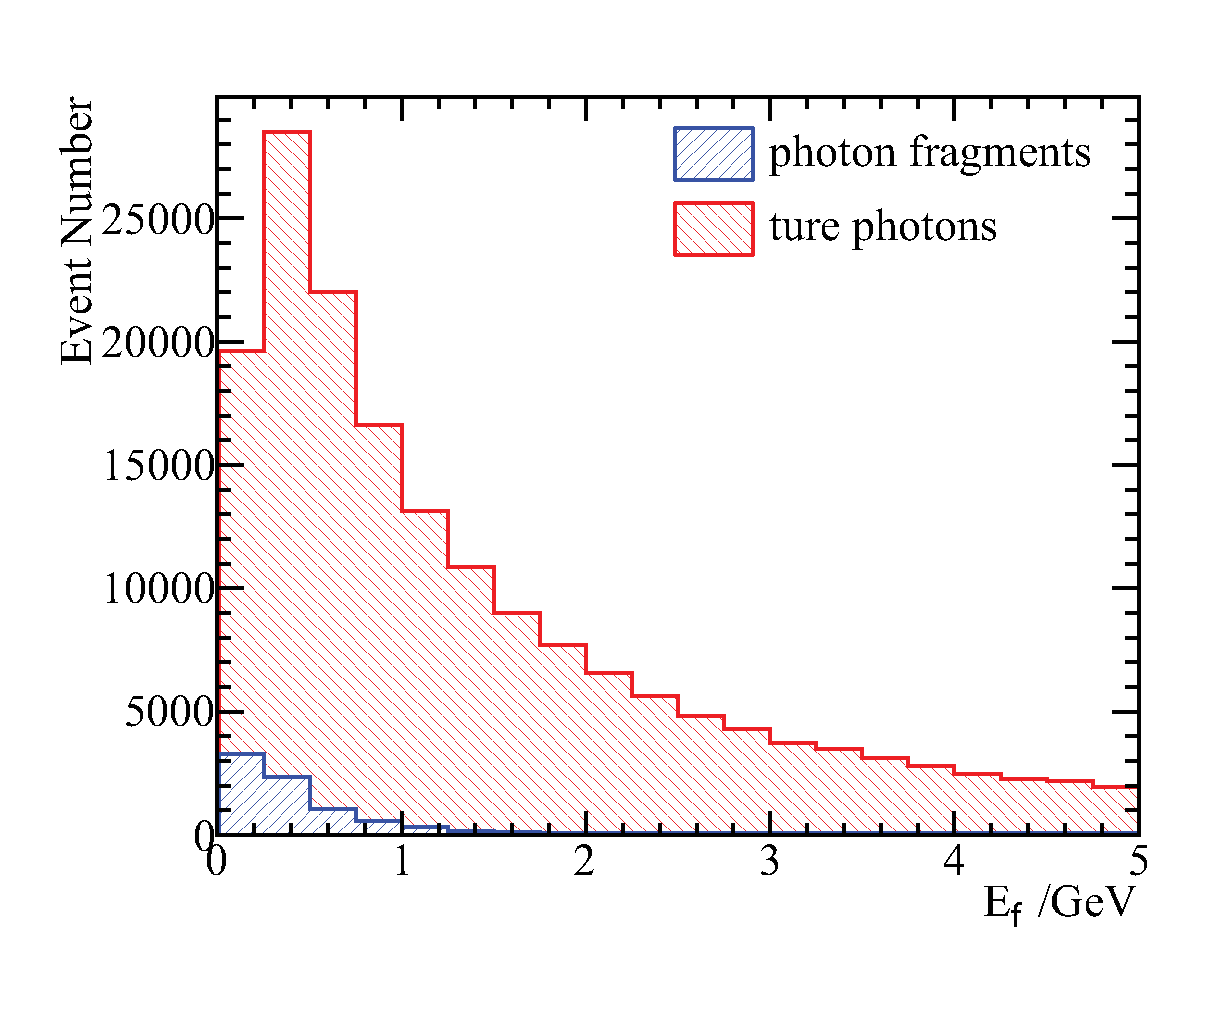
\includegraphics[width=\textwidth]{{photon/frag/Photon_e_2_pp}}
    \caption{}
    \label{fig:photonFragPhotonEnergy}
  \end{subfigure}
  \begin{subfigure}[b]{0.45\textwidth}
    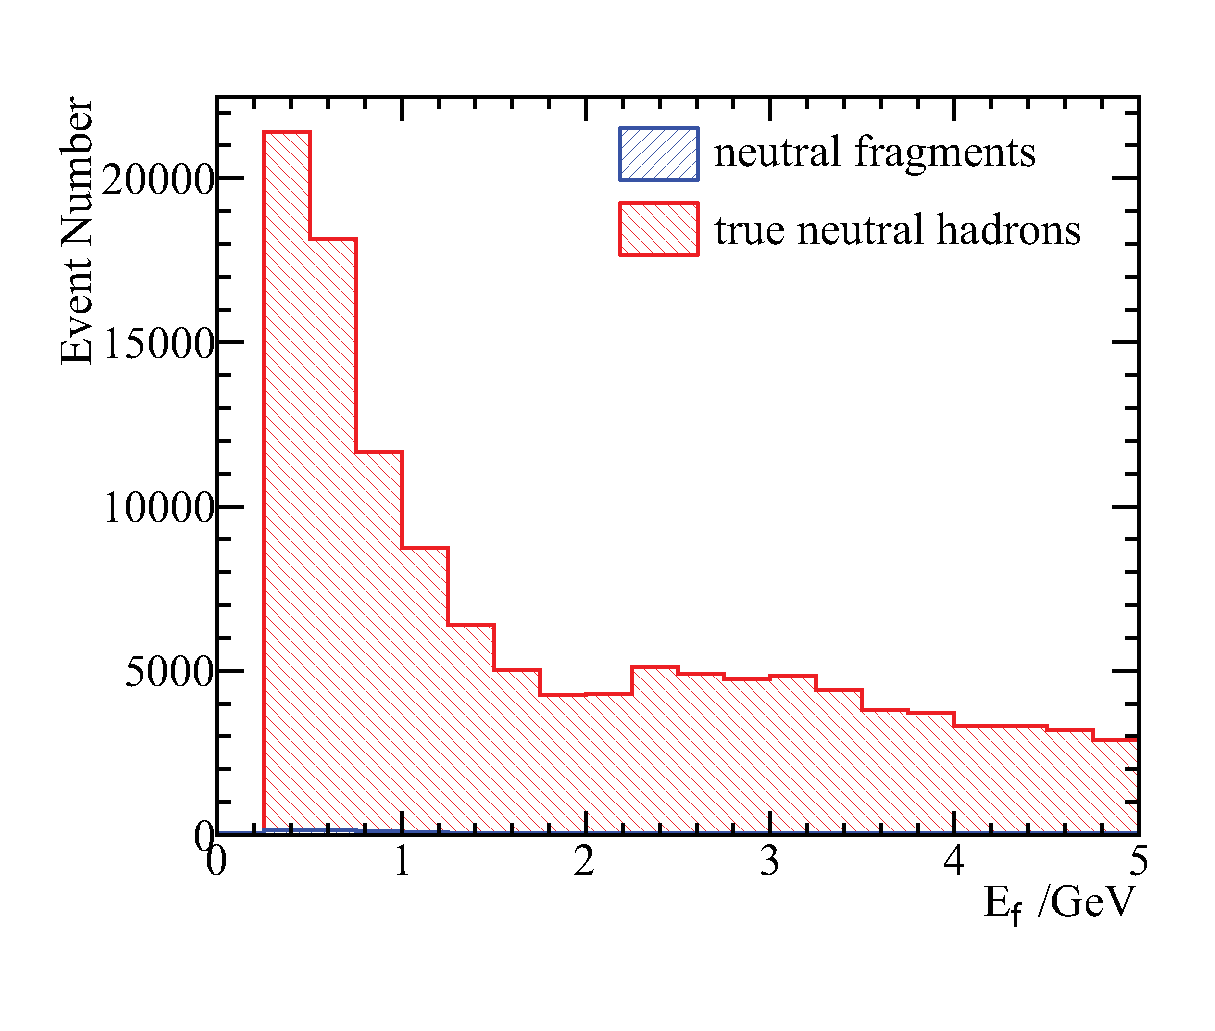
\includegraphics[width=\textwidth]{{photon/frag/Photon_e_2_pn}}
    \caption{}
    \label{fig:photonFragNeutralEnergy}
  \end{subfigure}
\caption
{The energies of the second most energetic reconstructed photons in the pair, for a) the photon$-$photon-fragment pairs, and the true photon$-$photon pairs , and for b) the  photon$-$neutral-hadron-fragment pairs, and the true photon$-$neutral-hadron pairs. Events were generated with \eeZuds, at \rootSGeV{500}, reconstructed with the \pandora version 1.}
\label{fig:photonFragEnergy}
\end{figure}


% , because they have different kinematic and topological distributions.
% $d$, $d_c$ and $d_h$ are mean energy weighted intra-layer distance within the pair, distance between two centroids, and minimum distance between calorimeter hits of each \PFO in the pair, respectively.  Three distance measurements have subtle difference.
There are two variants of the photon fragment removal algorithms: one immediately after the \PhotonReconstruction algorithm, and the other one after the charged particle reconstruction. Since two algorithms share same logics for fragment removal, the algorithm used   after the charged particle reconstruction will be discussed in detail here. \TABLE{tab:photonFragRemovalCuts} lists cuts for merging photon$-$photon-fragment pairs and photon$-$neutral-hadron-fragment pairs for both low energy and high energy fragments. The description of each variable used in the cuts will be provided first, followed by the descriptions of the logics of the cuts.



\subsection{Variables}

There are three distance variables: the variable $d_c$ gives the distance between centroids of the particles in the photon$-$fragment pair, which is a computationally quick measurement;  the variable  $d_h$ is the minimum distance between calorimeter hits of each particle in the photon$-$fragment pair;  the variable  $d$ is the average energy weighted intra-layer distance between  two particles in the photon$-$fragment pair, illustrated schematically in \Figure{fig:photonDistanceMetric}:
\begin{equation}
d = \frac{\sum_{i}^{layers}d_l^i \ E_{f}^i}{\sum_{i}^{layers}E_{f}^i}
\end{equation}
where index $i$ indicates $i^{th}$ layer of the \ECAL; the parameter $d_{l}^i$ is the minimum distance between calorimeter hits of the photon and the fragment in the $i^{th}$ layer; and $E_{f}^i$ is the total energy of calorimeter hits of the fragment in the $i^{th}$ layer of the \ECAL.

% All three distance metrics should be small to merge a photon$-$fragment pair.
%$d$ is a better measurement of the closeness of the pair.
\begin{figure}[tbph]
\centering
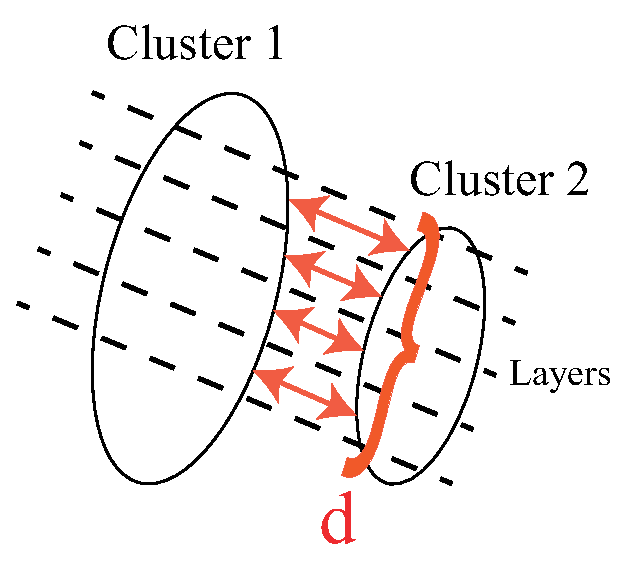
\includegraphics[width=0.35\textwidth]{photon/dLayer2}
\caption{An illustration of  the average energy weighted intra-layer distance between  two particles in the photon$-$fragment pair, $d$.}
\label{fig:photonDistanceMetric}
\end{figure}

\FIGURE{fig:photonFragPhotonLowD} and \Figure{fig:photonFragPhotonHighD} show the average energy weighted intra-layer distance between  each particle in the  photon$-$fragment pair ($d$) for  low-energy-fragment photon$-$photon-fragment pairs and the true photon$-$photon pairs, and high-energy-fragment photon$-$photon-fragment pairs and the true photon$-$photon pairs, respectively. \FIGURE{fig:photonFragNeutralLowDc} and \Figure{fig:photonFragNeutralHighDc} shows the distance between centroids between  each particle in the  photon$-$fragment pair for  low-energy-fragment photon$-$neutral-hadron-fragment pairs and the true photon$-$neutral-hadron pairs, and  high-energy-fragment photon$-$neutral-hadron-fragment pairs and the true photon$-$neutral-hadron pair, respectively. Events were generated with \eeZuds, at \rootSGeV{500}, reconstructed with the \pandora version 1.  Photon$-$fragment pairs typically have a small distance separation between the two particles.


\begin{figure}[tbph]
\centering
  \begin{subfigure}[b]{0.45\textwidth}
    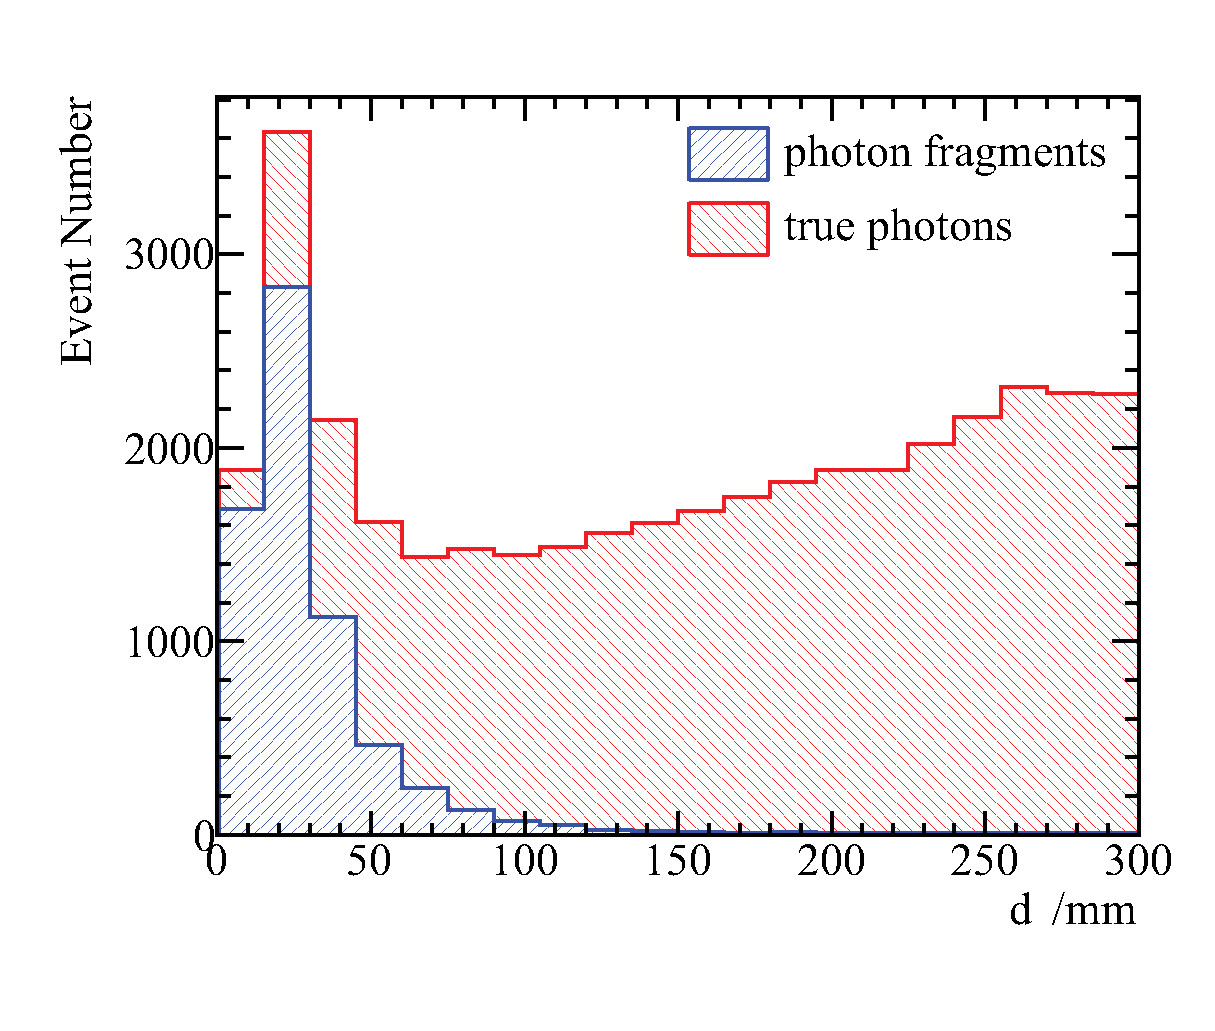
\includegraphics[width=\textwidth]{{photon/frag/Photon_d_low_pp}}
    \caption{}
    \label{fig:photonFragPhotonLowD}
  \end{subfigure}
  \begin{subfigure}[b]{0.45\textwidth}
    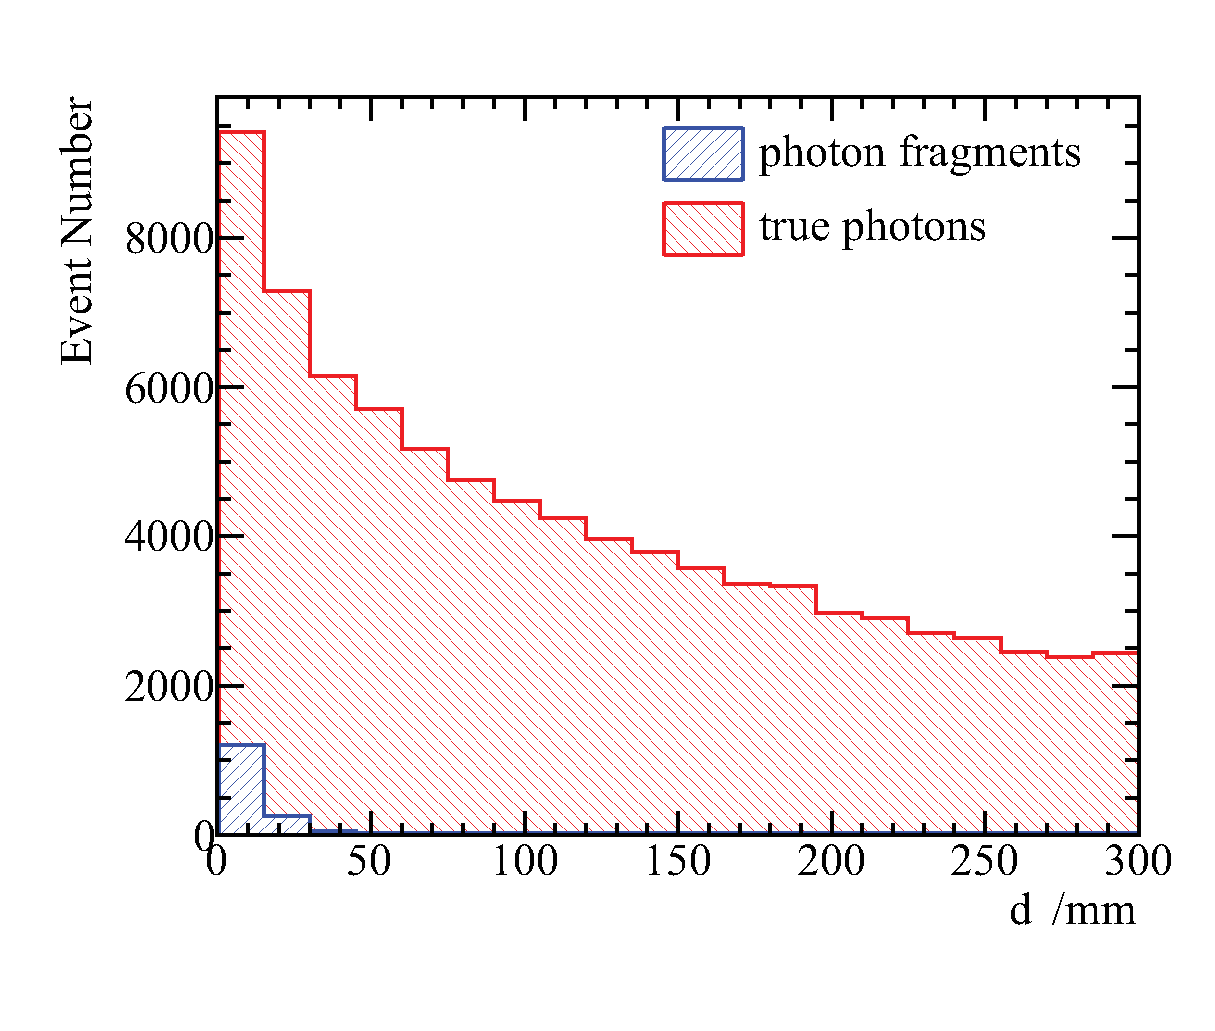
\includegraphics[width=\textwidth]{{photon/frag/Photon_d_hi_pp}}
    \caption{}
    \label{fig:photonFragPhotonHighD}
  \end{subfigure}
  \begin{subfigure}[b]{0.45\textwidth}
    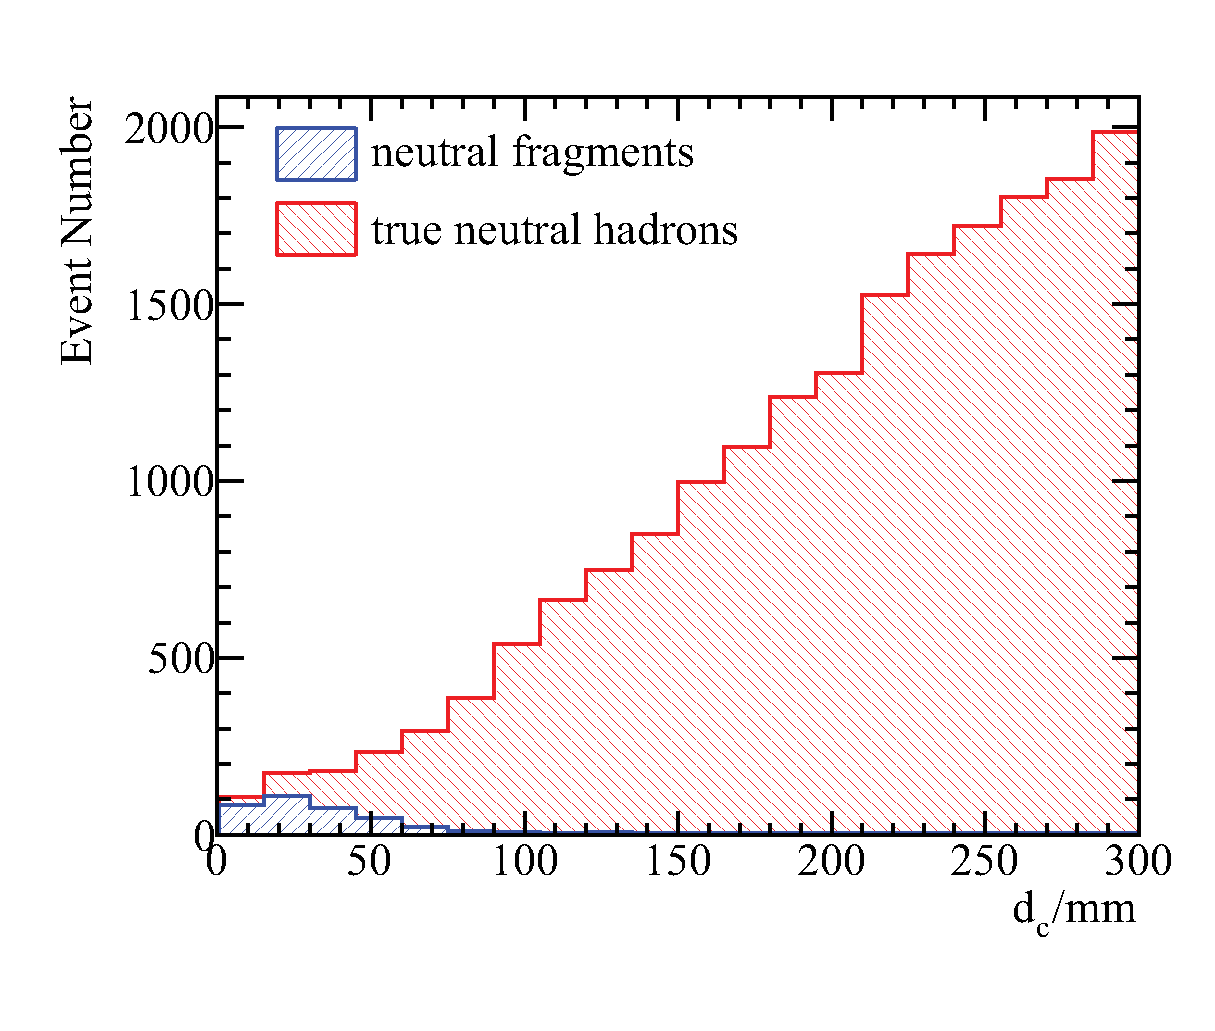
\includegraphics[width=\textwidth]{{photon/frag/Photon_dc_low_pn}}
    \caption{}
    \label{fig:photonFragNeutralLowDc}
  \end{subfigure}
  \begin{subfigure}[b]{0.45\textwidth}
    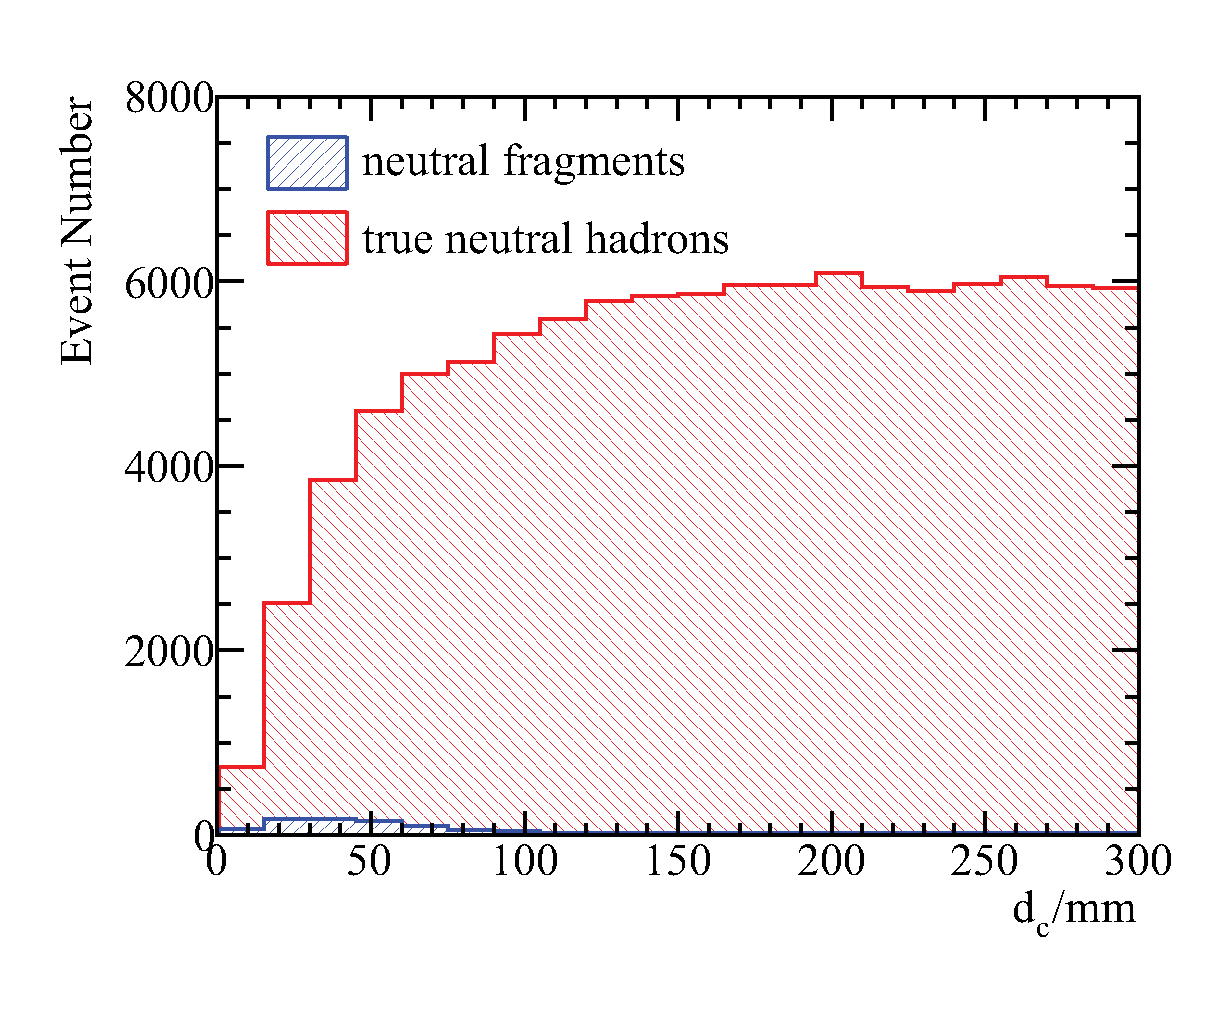
\includegraphics[width=\textwidth]{{photon/frag/Photon_dc_hi_pn}}
    \caption{}
    \label{fig:photonFragNeutralHighDc}
  \end{subfigure}
\caption
{Average energy weighted intra-layer distance between  each particle in the pair ($d$) for a) low-energy-fragment photon$-$photon-fragment pairs and the true photon$-$photon pairs, b) high-energy-fragment photon$-$photon-fragment pairs and the true photon$-$photon pairs. Distance between centroids between  each particle in the pair for c) low-energy-fragment photon$-$neutral-hadron-fragment pairs and the true photon$-$neutral-hadron pairs, b) high-energy-fragment photon$-$neutral-hadron-fragment pairs and the true photon$-$neutral-hadron pairs. Events were generated with \eeZuds, at \rootSGeV{500}, reconstructed with the \pandora version 1.}
\label{fig:photonFragDistance}
\end{figure}


Other quantities used in the merging metric include: $E_m$, the energy of the main photon; $E_f$,  the energy of the fragment; $E_{p1}$ and $E_{p2}$, the energies of the two most energetic EM showers,  identified by the \peakFinding algorithm, ordered by descending energy, using the photon$-$fragment pair as input; $N_{calo}$, the number of the calorimeter  hits in \ECAL in the fragment; and $\absCosTheta$, the absolute value of the cosine of the polar angle of the main photon with respect to the beam direction.

using the cuts for photon$-$photon-fragment with fragment energy $<$ 1\,GeV as an example,  each set of logics for merging fragments is discussed, Fragments passing any one set of cuts will be merged.

%The values used in the cuts are listed in \Table{tab:photonFragRemovalCuts}.

\subsection{Cuts}
%\subsection{Transverse shower comparison cuts}

The transverse shower comparison cut merges fragments when the photon$-$fragment pair looks like one EM shower in the two-dimensional energy deposition projection. The transverse shower comparison requires $\frac{E_{p1}}{E_m + E_f} > 0.9 $, demanding  most energy of the cluster contains in the most energetic peak found by the  \peakFinding algorithm. It also demands that the second energetic peak should have less than half of the energy in the fragment,  $\frac{E_{p2}}{E_f} < 0.5 $. And the most energetic peak should have more energy than the main photon,   $E_{p1} > E_m$. Lastly the fragment should be close to the main photon, $d < 30 $\,mm.
%One logic for merging is when

%The other logic of merging is when

%\subsection{Close proximity cuts}

The close proximity cut merges fragments  is when the fragment has a low energy and is spatially close to the main photon: $d < 20 $\,mm and the energy of the fragment is less than 0.2\,GeV.
%This set of cuts merges fragments if it is very close to the main photon and the fragment has a low energy.

%\subsection{Low energy fragment cuts}

%Another logic for merging  is when the fragment has a low energy and is spatially close to the main photon: $d < 20 $\,mm and the energy of the fragment is less than 0.2\,GeV.

% \subsection{Small fragment cuts}
% Two sets of cuts are developed.
The third set of logics, small fragment cuts,  for merging is when fragments that are spatially close to the main photon and have very few number of associated calorimeter hits. Either the  photon$-$fragment pair satisfies:  $d < 30 $\,mm; $d_c < 50 $\,mm; and number of calorimeter hits in the fragment less than 40. Or the  photon$-$fragment pair satisfies: $d < 30 $\,mm, and number of calorimeter hits in the fragment less than 50. The multiple sets of cuts allow the merging of a fragment with fewer number of  calorimeter hits with a slightly larger distance separation to the main photon, or the merging of a fragment with a slightly bigger number of  calorimeter hits with a smaller distance separation to the main photon.

%\subsection{Small fragment forward region cuts}
Another logic merges low-energy fragment in the  end cap region of the detector. The cut demands: $d_c < 60$\,mm; $\absCosTheta > 0.7$; the energy of the fragment less than 0.6\,GeV; and the number of calorimeter hits in the fragment less than 40.

%\subsection{Relative low energy fragment cuts}

The last merging logic is that the merged fragment should be relatively low energetic. The distance between the pair should satisfies $d < 40$\,mm and $d_h < 20$\,mm. The ratio of the fragment energy  to the main photon energy should be less than 0.01.
%$d < 40$\,mm; $d_h < 20$\,mm; $\frac{E_{f}}{E_m} < 0.01$

% If the fragment is close to the photon, and it is relative low energy to the photon, then the fragment is merged to the photon. This logic contains multiple sets of cuts, allowing the merging of a fragment with a smaller fragment-to-photon energy ratio with a slightly larger distance separation to the main photon, or the merging of  a fragment with a slightly higher  fragment-to-photon energy ratio with a smaller distance separation to the main photon.


%One logic of merging is when the fragment has low energy and is close to the main photon. Hence $E_f$  and $N_{calo}$ are required to be small. Alternatively the fragment should be relatively low energetic, demanding a small ratio of $E_f$ to $E_m$.




Cuts for high-energy fragments ($E_f>$1\,GeV) only has logics for transverse shower comparison and relative low energy fragment, as the cut on the absolute low-energy fragment is not applicable for the  high-energy fragments.

Neutral hadron fragments originated from charged particles are more likely to have low energies, but high-energy neutral hadron fragments are more likely to be originated from photons. Hence cuts for photon$-$neutral-hadron-fragment pair for low-energy fragment only merge fragments that are very close to the main photon, with very few calorimeter hits, or has a relative very small energy. The cuts for photon$-$neutral-hadron-fragment pair for high-energy fragment, on the other hand, are more generous, allow merging fragments that have energies of up to 20\% of the main photon energy.


%are similar. They differs in the values for cuts as the cuts for high energy fragments allow higher energy fragments to be merged.

%Comparing cuts for photon$-$photon-fragment pair and photon$-$neutral-hadron-fragment pair, the differences are in the values of cuts  due to the fact that  the neutral hadron fragments originated from charged particles are more likely to have low energies, and high-energy neutral hadron fragments are more likely to be originated from photons.

This merging test is iterated over all possible  photon$-$fragment pairs. If multiple photon$-$fragment pairs with the same photon pass the merging test, the pair with the smallest distance metric, $d$, will be merged.

Since all possible photon$-$fragment pairs are tested, this is a costly cooperation with $O(n^2)$ time complexity for $n$ particles. The speed is improved by considering only pairs with $d<80\ \text{mm}$.




\subsection{Photon fragment removal algorithm after the \PhotonReconstruction algorithm}

The photon fragment removal algorithm immediately after the \PhotonReconstruction algorithm shares the same logics as the stated above. The cuts for merging fragments are listed in \Table{tab:photonFragRemovalCuts2}.

%differs sightly in the values of the cuts, which
% The algorithm have stricter cuts as it is careful not to make mistakes at merging fragments.

\section{Photon fragment removal algorithm in the \HCAL}
\label{sec:photonHighEFragRemoval}

%The previous section describes  algorithms to remove photon fragments in the \ECAL that are peripheral to the electromagnetic shower core.

There is another type of fragments originated from the leakage effect of the \ECAL. When a high-energy EM shower is not fully contained in the \ECAL, the shower deposits energy in the \HCAL, which often forms a neutral hadron in the \HCAL. An example of a 500\,GeV photon reconstructed into a main photon in the \ECAL (yellow) and a neutral hadron fragment in the \HCAL (blue) is shown in \Figure{fig:photonEvtDspHCalFrag}. This section presents an algorithm to merge fragments in the \HCAL to the main photon.

%This photon fragment recovery algorithm is important when reconstructing  high energy photons.

%For the \ILD detector, this \ECAL leakage effect appears when the photon energy is above 50\,GeV.

\begin{figure}[tbph]
\centering
{
\includegraphics[width=0.5\textwidth]{photon/hcalfrag}}%
\caption{An event display of a typical 500\,GeV photon, reconstructed into a main photon in the \ECAL (yellow) and a neutral hadron fragment in the \HCAL (blue).}
\label{fig:photonEvtDspHCalFrag}
\end{figure}

Photon fragments in the \HCAL are  spatially close to the main photon. A cone obtained from fitting the main photon, if extended to the \HCAL, should contain most of the calorimeter hits of the fragment. These features allow a set of cuts developed to merge  fragments in the \HCAL, which are listed in \Table{tab:photonHighEnergyFragCuts}.


This algorithm uses photons in the \ECAL and neutral hadrons in the \HCAL as inputs. The algorithm then iterates over all pairs of reconstructed photons and neutral hadrons. Photon$-$fragment pairs passing all the cuts will be merged.

%For each pair, variables are calculated and compared to a set of cuts.

%\subsection{Adjacent in layers cut}

The adjacent in layers cut demands that  photon cluster deposit energies in the last outer layer of the \ECAL   and  the fragment deposits energies in the first inner layer of the \HCAL.

%\subsection{Energy comparison cut}


Another requirement for merging, energy comparison cut,  is that the fragment should have a low energy relative to the main photon. The variables $E_m$ and $E_f$ are the energy of the main photon  and the energy of the fragment, respectively. The ratio, $\frac{E_f}{E_m}$, has to be less than 0.1 for merging.



\FIGURE{fig:photonHCalFragCut1} shows the distributions of  the energy fractions ($\frac{E_f}{E_m}$) after passing the adjacent in layers cut, for photon fragments in jet samples (blue), non-fragments in jet samples (orange), and photon fragments in one-photon-per-event samples (green). Jet samples are \eeZuds, at \rootSGeV{500}, reconstructed with the \pandora version 1. One-photon-per-event samples are single 500\,GeV photon samples,  reconstructed with the \pandora version 1. The cut $\frac{E_f}{E_m}$ < 0.1 contains most of the fragments.


\begin{figure}[tbph]
\centering
{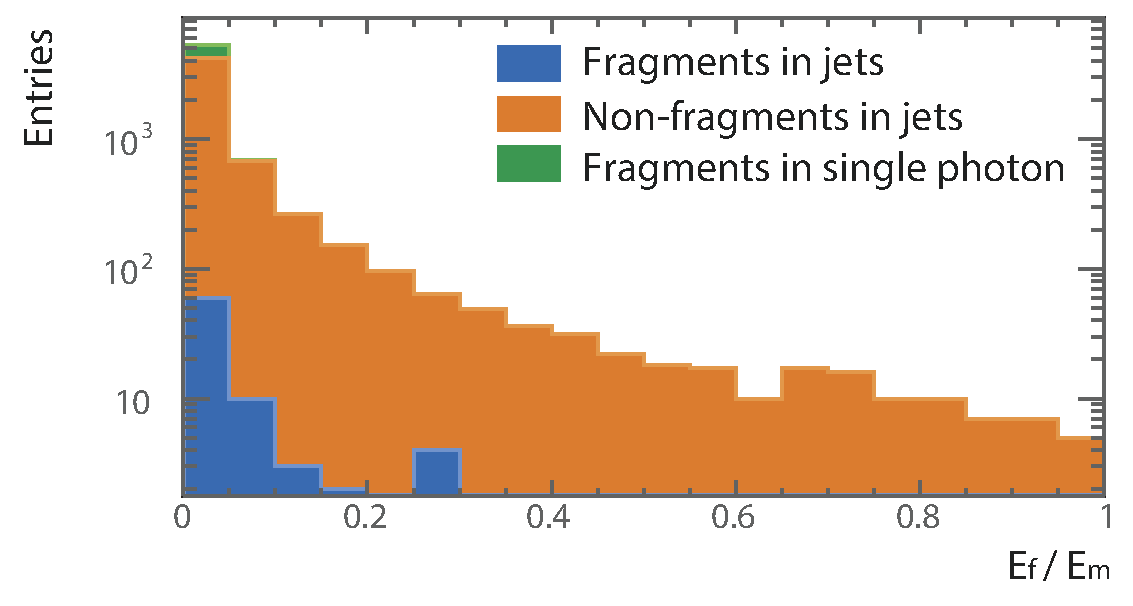
\includegraphics[width=0.7\textwidth]{{{photon/high/cutEhcalEecal0.1v2}}}}%
\caption{The stacked distributions of the energy fractions ($\frac{E_f}{E_m}$) after passing the adjacent in layers cuts, for photon fragments in jet samples (blue), non-fragments in jet samples (orange), and photon fragments in one-photon-per-event samples (green). Jet samples are \eeZuds, at \rootSGeV{500}, reconstructed with the \pandora version 1. One-photon-per-event samples are single 500\,GeV photon samples,  reconstructed with the \pandora version 1.}
\label{fig:photonHCalFragCut1}
\end{figure}



%\subsection{Distance comparison cuts}

The distance comparison cuts requires that fragments in the \HCAL to be merged to main photons  should be spatially close to the main photons, measured by three distance metrics: the variable $d^l_c$ is the distance between the centroid position of the calorimeter hits of the main photon in the last outer layer in the \ECAL, and the centroid position of the calorimeter hits of the fragment in the first inner layer of the \HCAL; the variable $d^l_{fit}$ is the shortest distance between the direction fitted with the calorimeter hits of the main photon in the  last outer layer in the \ECAL, and the direction fitted with  the calorimeter hits of the fragment in the first inner layer of the \HCAL; and $d_{fit}$ is the shortest distance between the direction fitted with the main photon, and the direction fitted with the fragment. These three distances should be small for merging. The cuts demand: $d^l_c \leqslant 173\,\text{mm}$; $d^l_{fit} \leqslant 100\,\text{mm}$; and $d_{fit} \leqslant 100\,\text{mm}$.

 \FIGURE{fig:photonHCalFragCut2} shows the distributions of ${d^l_c}^2$  after passing the adjacent in layers cut and the energy comparison cut, for photon fragments in jet samples (blue), non-fragments in jet samples (orange), and photon fragments in one-photon-per-event samples (green). The cut at  $d^l_c \leqslant 173$\,mm (${d^l_c}^2 \leqslant 3000$\,\uprightMath{mm^2}) covers most of the fragments.

  %Jet samples are \eeZuds, at \rootSGeV{500}, reconstructed with the \pandora version 1. One-photon-per-event samples are single 500\,GeV photon samples,  reconstructed with the \pandora version 1.

\begin{figure}[tbph]
\centering
{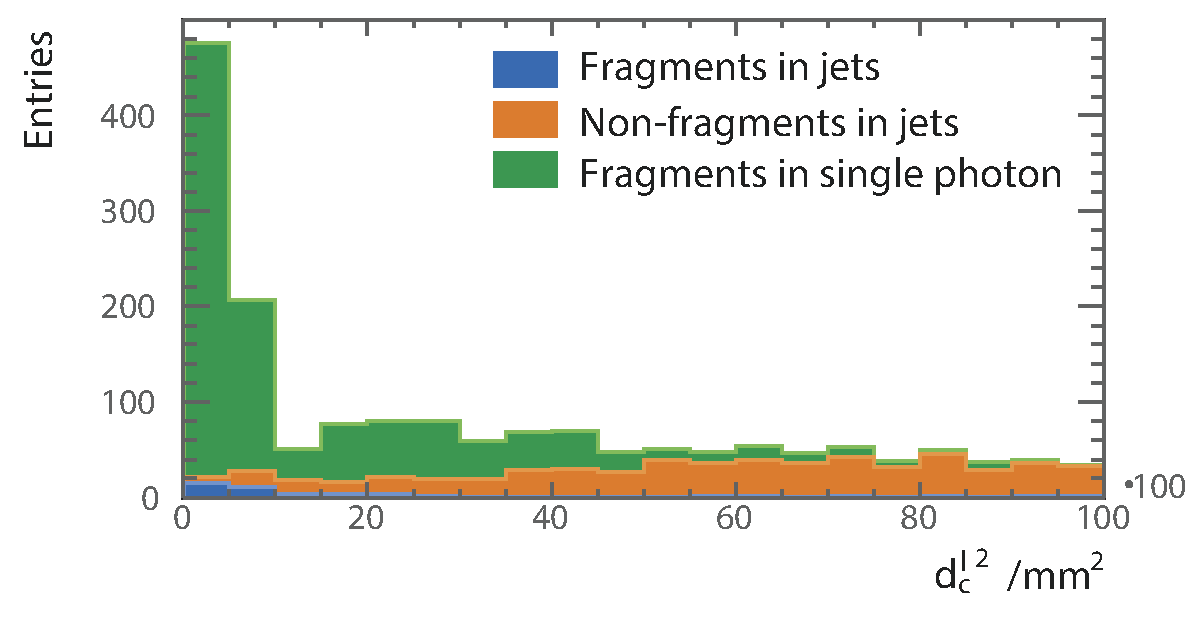
\includegraphics[width=0.7\textwidth]{{photon/high/cut2CentroidDistanceSqu30000v2}}}%
\caption{The stacked distributions of ${d^l_c}^2$ after passing the adjacent in layers cuts and the energy comparison cuts, for photon fragments in jet samples (blue), non-fragments in jet samples (orange), and photon fragments in one-photon-per-event samples (green). Jet samples are \eeZuds, at \rootSGeV{500}, reconstructed with the \pandora version 1. One-photon-per-event samples are single 500\,GeV photon samples,  reconstructed with the \pandora version 1.}
\label{fig:photonHCalFragCut2}
\end{figure}



%\subsection{Projection comparison cut}
The projection comparison cut states that the direction of the fragment  to be merged to the main photon should be similar to the direction of the main photon. The variable  $r_f$ is the energy weighted \rms  distance of a calorimeter hit in the fragment to the direction fitted with the main photon.  The cut requires $ r_f \leqslant 45\,\text{mm}$.

%\subsection{Shower width comparison cut}
The shower width comparison cut requires that the shower width of the fragment to be merged to the main photon  and the shower width of the main photon are similar. Variable $w^l_m$ is the \rms distance of the calorimeter hits of the main photon in last outer layer  in the \ECAL to the centroid of the calorimeter hits in the same layer. Variable  $w^l_f$ is the  \rms distance of the calorimeter hits of the fragment in the first inner layer  in the \HCAL to the centroid of the calorimeter hits in the same layer. The ratio $\frac{w^l_f}{w^l_m}$ needs to be in the range from 0.3 to 5 to pass the cut. The generous upper bound is because the \HCAL cell size is much larger than the cell size of the \ECAL.

%\subsection{Cone comparison cut}

The last cut, the cone comparison cut, demands that when a cone obtained by fitting the main photon in the \ECAL is extended to the fragment in the \HCAL, the cone should contain a significant amount of the fragment. The variable, $\frac{N_{cone}}{N_f}$, the fraction of the calorimeter hits in the fragment in the cone comparing to the  calorimeter hits in the fragment, has to be greater than 0.5 for merging.



\begin{table}[htbp]
\centering

\smallskip

\begin{tabular}{l r }
\hline
\hline
Photon fragment recovery&  Cuts\\
\hline
\multicolumn{1}{L{0.3\textwidth}}{Adjacent in layers} & \multicolumn{1}{R{0.6\textwidth}}{yes} \\
\multicolumn{1}{L{0.3\textwidth}}{Energy comparison} & \multicolumn{1}{R{0.6\textwidth}}{$ \frac{E_f}{E_m} \leqslant 0.1$} \\
\multicolumn{1}{L{0.3\textwidth}}{Distance comparison} & \multicolumn{1}{R{0.6\textwidth}}{$d^l_c \leqslant 173\,\text{mm}$; $d^l_{fit} \leqslant 100\,\text{mm}$; $d_{fit} \leqslant 100\,\text{mm}$} \\
\multicolumn{1}{L{0.3\textwidth}}{Projection comparison} & \multicolumn{1}{R{0.6\textwidth}}{$ r_f \leqslant 45\,\text{mm}$} \\
\multicolumn{1}{L{0.3\textwidth}}{Shower width comparison} & \multicolumn{1}{R{0.6\textwidth}}{$  0.3 \leqslant \frac{w^l_f}{w^l_m} \leqslant 5$} \\
\multicolumn{1}{L{0.3\textwidth}}{Cone comparison} & \multicolumn{1}{R{0.6\textwidth}}{$ \frac{N_{cone}}{N_f} \geqslant 0.5$} \\

\hline
\hline
\end{tabular}

\caption[Cuts for merging high energy photon fragment in the \HCAL.]%
{The cuts for merging high energy photon fragment in the \HCAL to the main photon in the \ECAL. }

%The variable $d^l_c$ is the distance between the centroid position of the calorimeter hits of the main photon in the last outer layer in the \ECAL and the centroid position of the calorimeter hits of the fragment in the first inner layer of the \HCAL. The variable $d^l_{fit}$ is the shortest distance between the direction fitted with the calorimeter hits of the main photon in the  last outer layer in the \ECAL and the direction fitted with  the calorimeter hits of the fragment in the first inner layer of the \HCAL. The variable $d_{fit}$ is the shortest distance between the direction fitted with the main photon and the direction fitted with the fragment. The variable  $r_f$ is the \rms energy weighted distance of a calorimeter hit in the fragment to the direction fitted with the main photon. Variables $w^l_m$ and $w^l_f$ are the \rms widths of the calorimeter hits of the main photon in last outer layer  in the \ECAL, and the calorimeter hit of the fragment in the first inner layer  in the \HCAL, respectively. Variable $\%{N}$ is the fraction of the calorimeter hits in the fragment in the cone comparing to the  calorimeter hits in the fragment.  Variables $E_m$ and $E_f$ are the energy of the main photon  and the energy of the fragment, respectively.
\label{tab:photonHighEnergyFragCuts}
\end{table}


If multiple photon$-$fragment pairs pass the cuts with the same fragment, the pair with highest $\frac{N_{cone}}{N_f}$ will be merged.

%This \HCAL fragment removal algorithm occurs after the first pass of topological association in the reconstruction which connects tracks to clusters in the calorimeters.


\section{Photon splitting algorithm}
\label{sec:photonSplitting}

%Algorithms described above deal with forming photons from calorimeter hits in the \ECAL, merging photon fragments in the \ECAL and the \HCAL.

Another aspect in photon reconstruction is to split accidentally merged photons. During the event reconstruction, it is possible that photons are accidentally merged if they are spatially close. Hence an algorithm at the end of the event reconstruction addresses this issue and tries to split merged photons.

%Merged photons are typically energetic.
If a photon has the  topology of multiple spatially closed photons, the parent photon should be split into several daughter photons. Extra care should be taken if the parent photon is close to a track projection onto the front of the \ECAL. \TABLE{tab:photonPhotonSplitting} lists the cuts used in the algorithm.

%This algorithm focuses on energetic photons with energies greater than 10\,GeV.
The algorithm works as follows. If an energetic photon is identified, the \peakFinding algorithm will  be used to identify EM showers in the parent photon. If energy of the parent photon is bigger than $E_{c1}$, and the energy of the $2^{nd}$ energetic EM shower is bigger than $E_{c2}$, the parent photon will be split to daughter photons according to the number of EM showers identified by the \peakFinding algorithm.

The values of $E_{c1}$ and $E_{c2}$ depend on whether the parent photon is close to a track projection onto the front of the \ECAL. The algorithm demands  higher values of $E_{c1}$ and   $E_{c2}$, if the photon is close to the track projection. The number of nearby charged tracks is counted as number of tracks with the track projection onto the front of the \ECAL fewer than 100\,mm to the parent photon centroid position. If there is no nearby tracks to the parent photon, $E_{c1}$ is set to 10\,GeV and $E_{c2}$ is set to 1\,GeV. If there is one nearby track, $E_{c1}$ is set to 10\,GeV and $E_{c2}$ is set to 5\,GeV. If there is more than one nearby track, $E_{c1}$ is set to 20\,GeV and $E_{c2}$ is set to 10\,GeV.


%energises of the photon and the second energetic EM shower
%When the candidate is close to a charged track, which is defined as within 100\,mm of the track projection on the front of the \ECAL, extra care is taken by demanding a large value for second EM shower energy. $E_{c1}$ and $E_{c2}$, the energy cut-off values, are determined by the number of nearby charged track.

The constraint on $N_{p}$, the number of EM showers identified in the parent photon, should be fewer than five, as one reconstructed photon is unlikely to be accidentally merged from more than four photons.


\begin{table}[htbp]
\centering
\smallskip
\begin{tabular}{l r }
\hline
\hline
Photon splitting&  Cuts\\
\hline
\multicolumn{1}{L{0.3\textwidth}}{Cuts} & \multicolumn{1}{R{0.6\textwidth}}{$E > E_{c1}$, $E_{p2} > E_{c2}$, $N_{p} < 5$} \\
\hline
$E_{c1}$ and $E_{c2}$ values &  \\
\hline
\multicolumn{1}{L{0.3\textwidth}}{0 track nearby} & \multicolumn{1}{R{0.6\textwidth}}{$E_{c1} = 10$\,GeV, $E_{c2} = 1$\,GeV} \\
\multicolumn{1}{L{0.3\textwidth}}{1 track nearby} & \multicolumn{1}{R{0.6\textwidth}}{$E_{c1} = 10$\,GeV, $E_{c2} = 5$\,GeV} \\
\multicolumn{1}{L{0.3\textwidth}}{> 1 tracks nearby} & \multicolumn{1}{R{0.6\textwidth}}{$E_{c1} = 20$\,GeV, $E_{c2} = 10$\,GeV} \\
\hline
\hline
\end{tabular}

\caption[Cuts for splitting photons.]%
{Cuts used in the photon splitting algorithm. The parameter $E$ is the energy of the parent photon. The parameter $E_{p2}$ is  energy of the second energetic peak obtained from \peakFinding algorithm. The parameter $N_{p}$ is the number of peaks identified by \peakFinding algorithm. The parameters $E_{c1}$ and $E_{c2}$ are the energy threshold values, determined by the number of nearby tracks to the parent photon.}
\label{tab:photonPhotonSplitting}
\end{table}

\section{Photon reconstruction performance}


%Motivations and implementations of four different photon related algorithms have been described above.

%The main photon reconstruction algorithm in \Section{sec:photonRecostrcution} improves the photon reconstruction, due to the improved \peakFinding algorithm in \Section{sec:peakFinding}. The fragment removal algorithms in \Section{sec:photonFragRemoval} and \Section{sec:photonHighEFragRemoval} reduce the photon fragments in the \ECAL and the \HCAL. The photon splitting algorithm in \Section{sec:photonSplitting} exploits the \peakFinding algorithms to separate photons using transverse shower information, which separates photons that   improves the photon separation resolution. Photon reconstruction improves single photon resolutions. It also improves jet energy resolution at a high centre-of-mass energy because of the high photon reconstruction completeness.

Three different versions of the \pandora are used to demonstrate the improvement of  the photon reconstruction performance:
\begin{itemize}
  \item with no stand-alone photon reconstruction algorithms,
  \item with a stand-alone photon reconstruction algorithm from \pandora version 1,
  \item with full photon related algorithms described above, incorporated in \pandora version 3,
\end{itemize}

Without photon reconstruction algorithms, \pandora applies a simple photon ID at the end of the event reconstruction. In \pandora version 1, there is a rudimentary photon reconstruction algorithm. In \pandora version 3 contains all the photon algorithms presented in this chapter, as the algorithms  were developed during \pandora version 2. Also in \pandora version 3, the photon algorithms  have replaced the   photon reconstruction algorithm in \pandora version 1.

Firstly the photon reconstruction performance with the full algorithms implemented in \pandora version 3 is compared with the performance with no photon algorithms. Afterwards, the photon reconstruction performance  is compared with the performance obtained from  \pandora version 1. The photon reconstruction performances of individual photon algorithms are then characterised, followed by the characterisation of the performance of the photon algorithms in \pandora version 3.

\subsection{Improvement from no photon algorithms}

The improvement in the photon reconstruction from no photon algorithms is demonstrated using  two-photon-per-event samples. The two-photon-per-event samples were generated with an uniform distribution in the solid angle of the first photon, and an uniform distribution in the opening angles  between the photon pair. Events were selected such that there is no early photon conversion in the tracking detector and the photon does not escape the detector undetected. The events are further restricted to photon decaying in barrel and endcap region only, to avoid the barrel/endcap overlap region. Events were reconstructed using the nominal \ILD detector model.

% the solid angle  for a range of

\FIGURE{fig:photonDoublePerformanceNoReco} shows the average number of reconstructed photons as a function of true distance separation between two photons,   using  two-photon-per-event samples
with photon energies of  500\,GeV and 50\,GeV,   reconstructed with and without photon algorithms. For the reconstruction without the photon algorithms, the number of photon fluctuates between 1 and 1.5 for a distance separation of 0 to 30\,mm between two photons.  For the reconstruction with the photon related algorithms, two photons start to be resolved at a distance separation  of 10\,mm between two photons, and fully resolved at 20\,mm distance separation.  The average number of reconstructed photon is 2 at 20\,mm distance separation.

% Without the photon related algorithms, the number of photon fluctuates between 1 and 1.5 for a distance separation of 0 to 30\,mm.  The number of photons between 0 and 5\,mm distance separation is 1.2. The true photon number for that distance separation should be 1, as it is challenging to separate photons less than one \ECAL cell size apart.

\begin{figure}[!tbph]
\centering
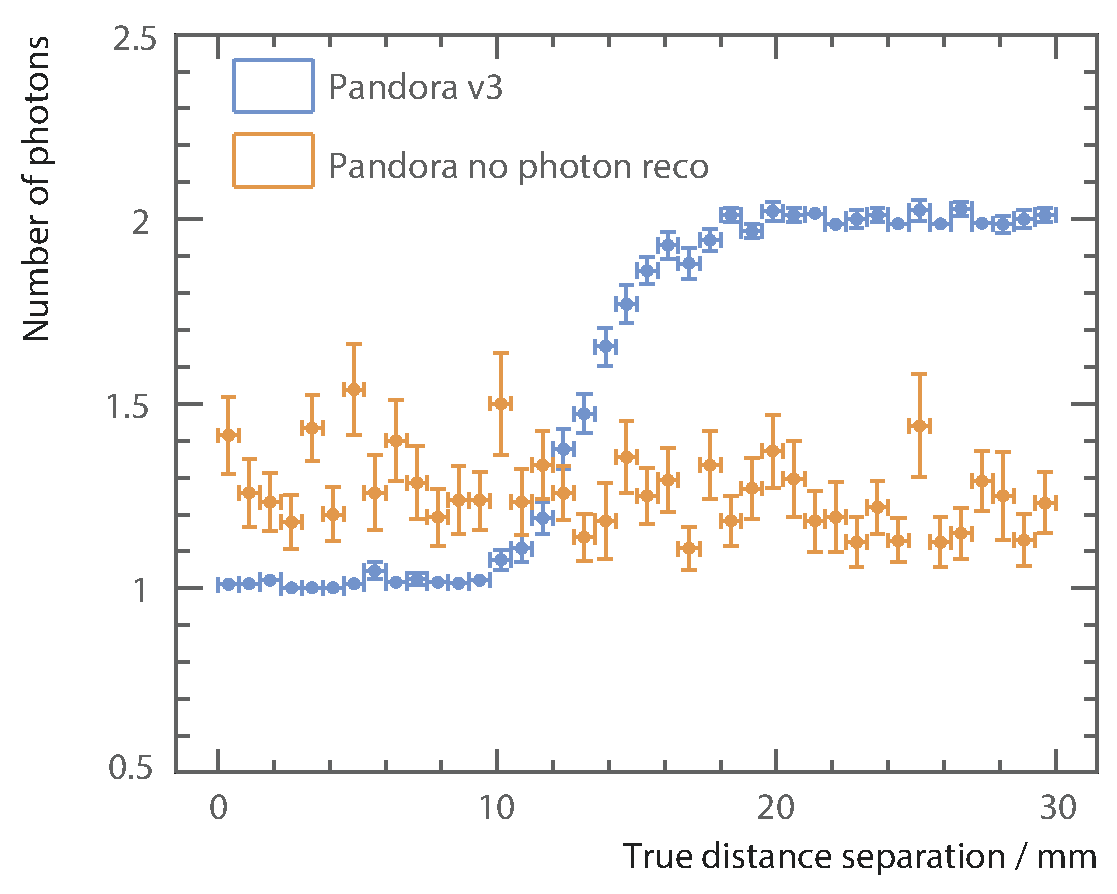
\includegraphics[width=0.85\textwidth]{photon/nPhotonVSnoPhotonReco3}
\caption[Average number of photons using two photons of 500 and 50\,GeV per event sample.]
{Average number of reconstructed  photons using two-photon-per-event samples with photon energies of  500\,GeV and 50\,GeV, without (orange) and with (blue) photon algorithms, as a function of the Monte Carlo distance separation between the photon pair.}
\label{fig:photonDoublePerformanceNoReco}
\end{figure}




The improvement in photon reconstruction leads to a considerable improvement in the jet energy resolution. Jet energy resolution is defined as the \rms divided by the mean for the smallest width of distribution that contains 90\% of entries, using \eeZuds, at barrel region. The angular cut is to avoid the barrel/endcap overlap region. The light quark decay of the \Zprime is used   to avoid the complication of missing momentum from semi-leptonic decay of heavy quarks. Using 90\% of the entries is robust and focus on the Gaussian part of the jet energy distribution. The total jet energies are   sampled at the centre-of-mass energies of 91, 200, 360 and 500\,GeV.

Shown in \Figure{fig:photonJERmuon}, the jet energy resolutions are much better at \rootSGeV{360} and 500\,GeV for the reconstruction with photon algorithms. By identifying photons before reconstructing charged particles in a dense jet environment, there are fewer calorimeter hits left for the charged particle reconstruction. However, at \rootSGeV{91} and 200\,GeV, the jet energy resolution are worse  for the reconstruction with photon algorithms, because photon algorithms are developed with  jet environments at a centre-of-mass energy of 500\,GeV.

\begin{figure}[!tbph]
\centering
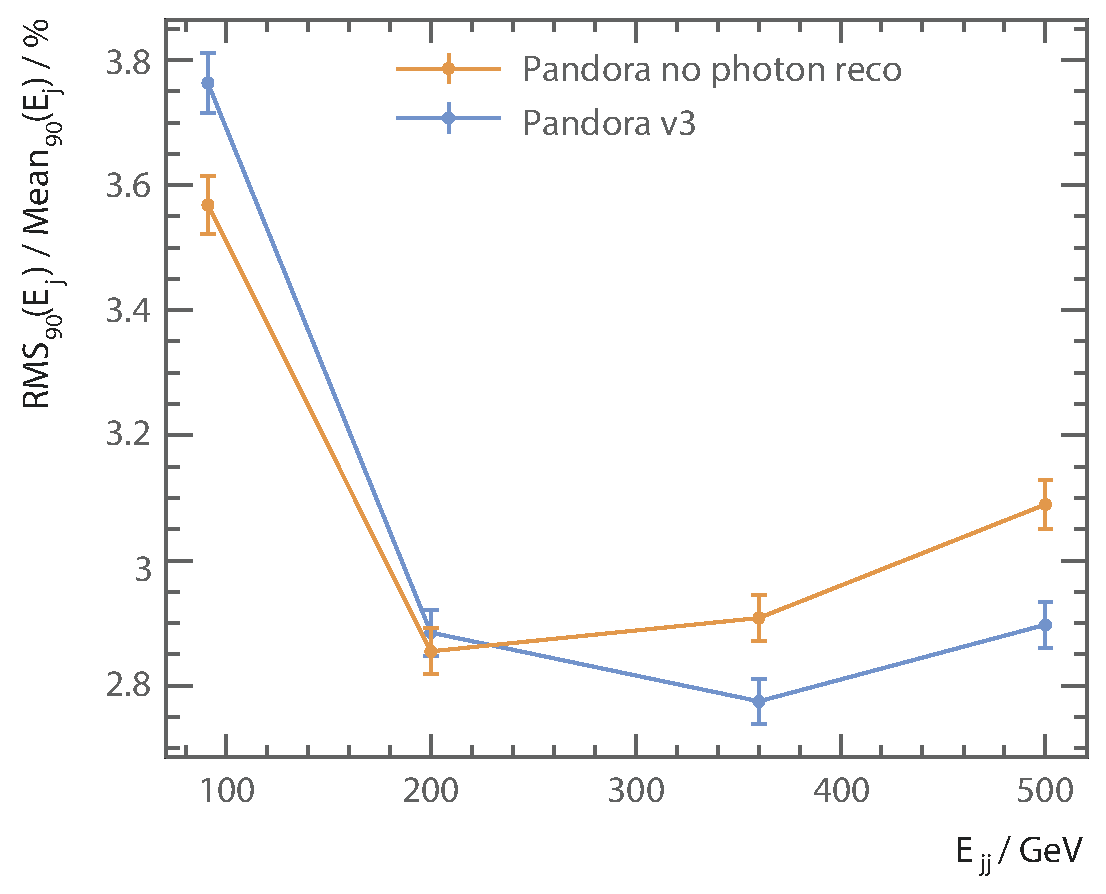
\includegraphics[width=0.85\textwidth]{photon/JERmuon2}
\caption[Jet energy resolution as a function of the total jet energy without and with photon related algorithms]
{Jet energy resolutions as a function of the  total jet energy using \eeZuds,  at barrel region. The orange and bottom dots represent the reconstruction without and with photon algorithms, respectively.}
\label{fig:photonJERmuon}
\end{figure}


The impact of photon algorithms on the jet energy resolution was studied using the same jet samples, reconstructed with the perfect photon reconstruction, which identifies photons by associating calorimeter hits using the truth information.  The photon confusion terms, which are defined as the quadrature differences of the jet energy resolutions between  a non-cheated reconstruction and a perfect photon reconstruction, are listed in \Table{tab:photonPhotonConfusion} for reconstruction with and without photon algorithms. The photon confusion terms, except at \rootSGeV{91}, have been reduced to 0.9\% for reconstruction with photon algorithms.


\begin{table}[htbp]
\centering
\begin{tabular}{ l   r  r  r  r   }
\hline
\hline
Photon confusion &\rootSGeV{91} & 200\,GeV & 360\,GeV & 500\,GeV  \\
\hline
\multicolumn{1}{L{0.3\textwidth}}{\pandora without photon algorithms}& 0.7\% & 0.9\% & 1.3\% & 1.4\%  \\
\multicolumn{1}{L{0.3\textwidth}}{\pandora with full photon algorithms} & 1.4\% & 0.9\% & 0.9\% & 0.9\%  \\
\hline
\hline
\end{tabular}

\caption[Photon confusion as a function of energy for reconstruction with and without photon algorithms.]
{Photon confusion terms as a function of total jet energies in the \eeZuds, for reconstruction with and without photon algorithms.}
\label{tab:photonPhotonConfusion}
\end{table}

\begin{comment}
    Double_t y2[nPoints] = {3.56892,2.85493,2.90771,3.08924};// MUON /r02/lc/xu/MarlinPandoraTest/HEAD20151210/20151211am10/
    Double_t erry2[nPoints] = {0.0460938,0.036756,0.0370356,0.0396873 };// MUON with 20150413 20150929am14

    //Double_t y2[nPoints] = {3.49641, 2.72426, 2.61667, 2.7686};// perfect photon from steve
    //Double_t erry2[nPoints] = {0.0444942,0.036756,0.0334291,0.0353562 };//


    Double_t y1[nPoints] = {3.76354,2.8844,2.77463,2.89704};// new photon with merging 20160107am13
    Double_t erry1[nPoints] = {0.0482638,0.0371727,0.0357569 ,0.03669   };//
\end{comment}

\subsection{Improvement from \pandora version 1}
\label{sec:photonPerformanceCompare}

This section reviews the photon reconstruction improvement  from \pandora version 1 to version 3, using single-photon-per-event, two-photon-per-event, and jet samples.

%The \ECAL square cell size is about 5\,mm.

%We will review performance metrics of above algorithms. \Fig{fig:n_p} shows the number of reconstructed photons as a function of their true distance separation for a two photons per event sample. The reduction of the number of reconstructed photons are mainly due the the fragment merging algorithms for fragments in the ECal. \Fig{fig:n_all} shows a similar reduction in the reconstructed particles as in \Fig{fig:n_p}, and it shows that neutral hadron fragments in HCal have been merged back to main photons.

The single-photon-per-event samples were generated with an uniform distribution in the solid angle of the photon. Other samples were generated and simulated in the same way as previously. The same selection as previously was applied to the  single-photon-per-event and  two-photon-per-event samples .

\FIGURE{fig:photonSingleN_p} shows the average number of reconstructed photons as a function of the true photon energies, using single-photon-per-event samples. Comparing the reconstruction with \pandora version 3 to version 1, for a 100\,GeV photon sample, the average number of reconstructed photons is reduced to 1 from 2; for a 500\,GeV photon sample, the  number is reduced to 1.05 from 2.8. \FIGURE{fig:photonSingleN_all} shows the average number of reconstructed particles as a function of the true photon energies, using single-photon-per-event samples. The number of  reconstructed particles counts the fragments reconstructed as neutral hadrons, as well as photons.   Comparing the reconstruction with \pandora version 3 to version 1,  for a 100\,GeV photon sample, the average number of reconstructed particles is reduced to 1 from 2.4; for a 500\,GeV photon sample, the number is reduced to 1.05 from 3.8.


%eduction in fragments reconstructed as photons,

%For the reconstruction in \pandora version 3, indicating as the blue dots on the plot, average number of photon stays below 1.05 for a photon energy of  500 \,GeV (true value 1).



%An  improvement in the number of reconstructed particles is shown in \Figure{fig:photonSingleN_all}. The number of  reconstructed particles counts the fragments reconstructed as neutral hadrons and photons.  Comparing \pandora version 3 with version 1, for a 100\,GeV photon sample, the average number of reconstructed particles is reduced to 1 from 2.4; for a 500\,GeV photon sample, the number is reduced to 1.05 from 3.8.


\begin{figure}[tbph]
\centering
    \begin{subfigure}[b]{0.45\textwidth}
        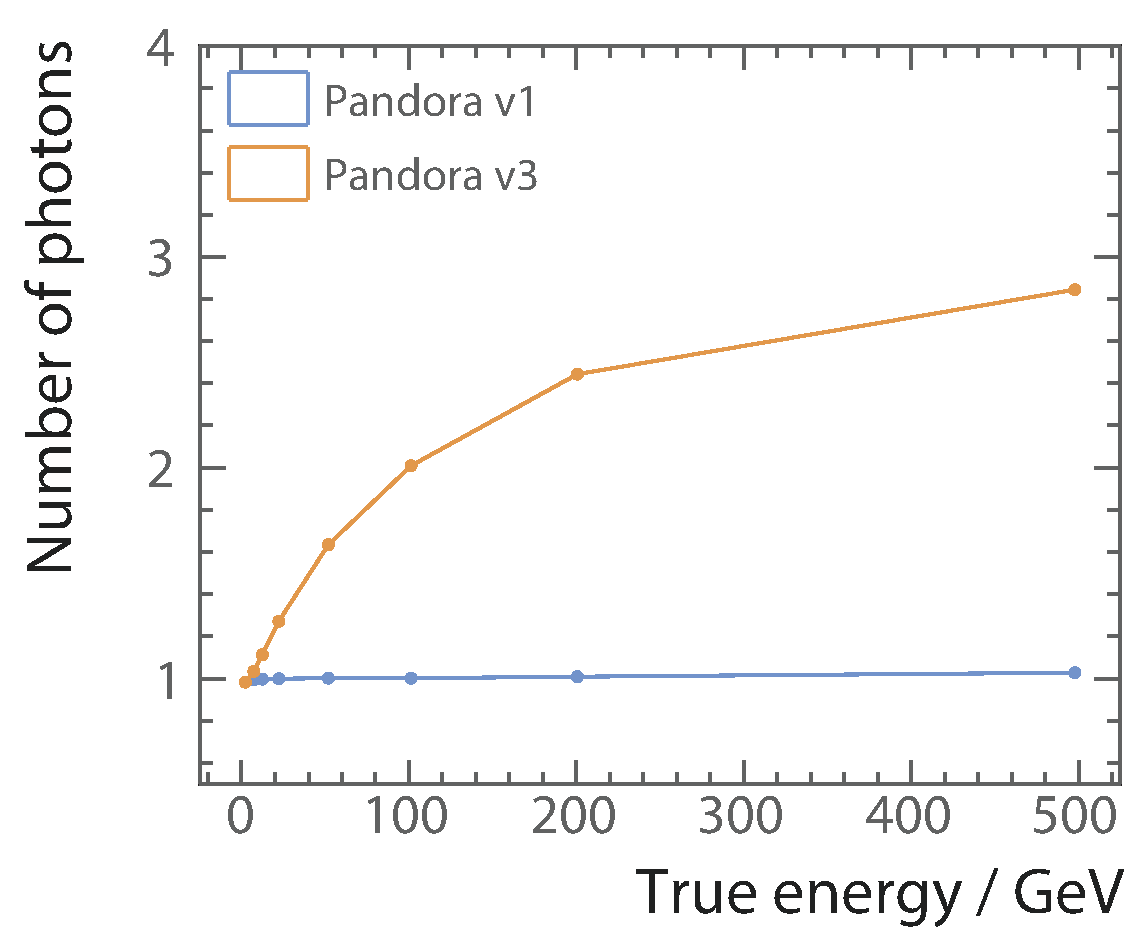
\includegraphics[width=\textwidth]{photon/SingleN_p2}
        \caption{}
        \label{fig:photonSingleN_p}
    \end{subfigure}
    \begin{subfigure}[b]{0.45\textwidth}
        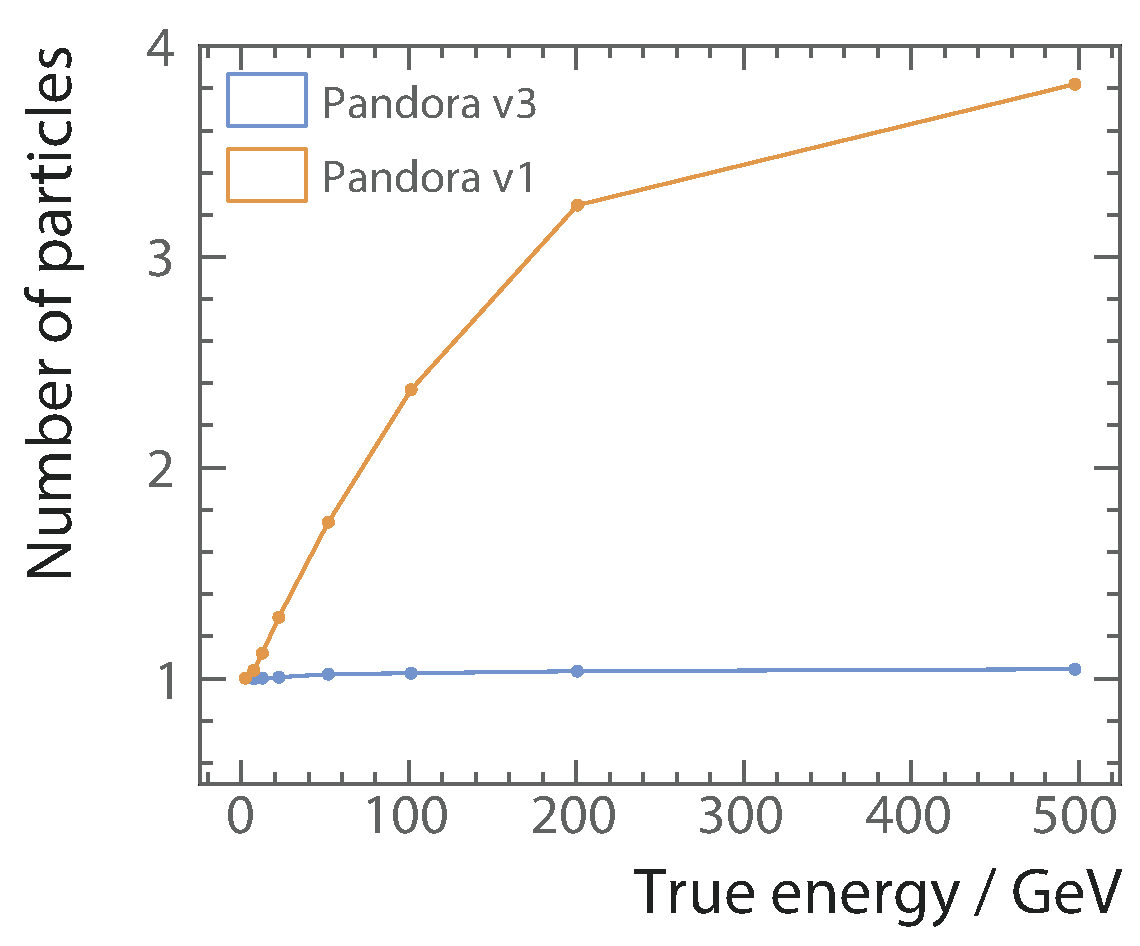
\includegraphics[width=\textwidth]{photon/SingleN_all2}
        \caption{}
        \label{fig:photonSingleN_all}
    \end{subfigure}
\caption[Average number of reconstructed photons and reconstructed particles, as a function of their true energy using single photon sample.]
{Average numbers of reconstructed a) photons, and b) particles, as a function of their true energies using  single-photon-per-event samples. For both figures, the top orange and bottom blue dots are reconstructed with \pandora version 1 and version 3, respectively.}
\label{fig:photonSingleN}
\end{figure}

%The photon reconstruction is changed in \pandora version 2.

\FIGURE{fig:photonDoubleCompareN} shows the numbers of reconstructed photon and particles as a function of  the true distance separation of the photon pair, using a two-photon-per-event sample with photon energies of  500\,GeV and 50\,GeV.  The average numbers of photon and particle for reconstruction with \pandora version 3 are both below 2.05 at 30\,mm distance apart, which is significantly lower than the numbers for reconstruction with \pandora version 1. For reconstruction with \pandora version 3, two photons start to be resolved at 10\,mm apart, and fully resolved at 20\,mm apart.


% from 0 to 30\,mm


% reduction in the photon fragments and the neutral hadron fragments using a two-photon-per-event sample with photon energies of  500\,GeV and 50\,GeV. The figures show the numbers of reconstructed photon and particles as a function of  the Monte Carlo distance separation of the photon pair from 0 to 30\,mm, which corresponds to approximately 6 \ECAL square cell lengths of the default \ILD detector model.

%This is a difficult test for fragment removal as high energy photons are more likely to create fragments. The imbalance in the two photon energies makes it more difficult to separate correctly, as the \peakFinding algorithm could not exploit the symmetry between two equally sized EM showers.

\begin{figure}[tbph]
\centering
    \begin{subfigure}[b]{0.45\textwidth}
        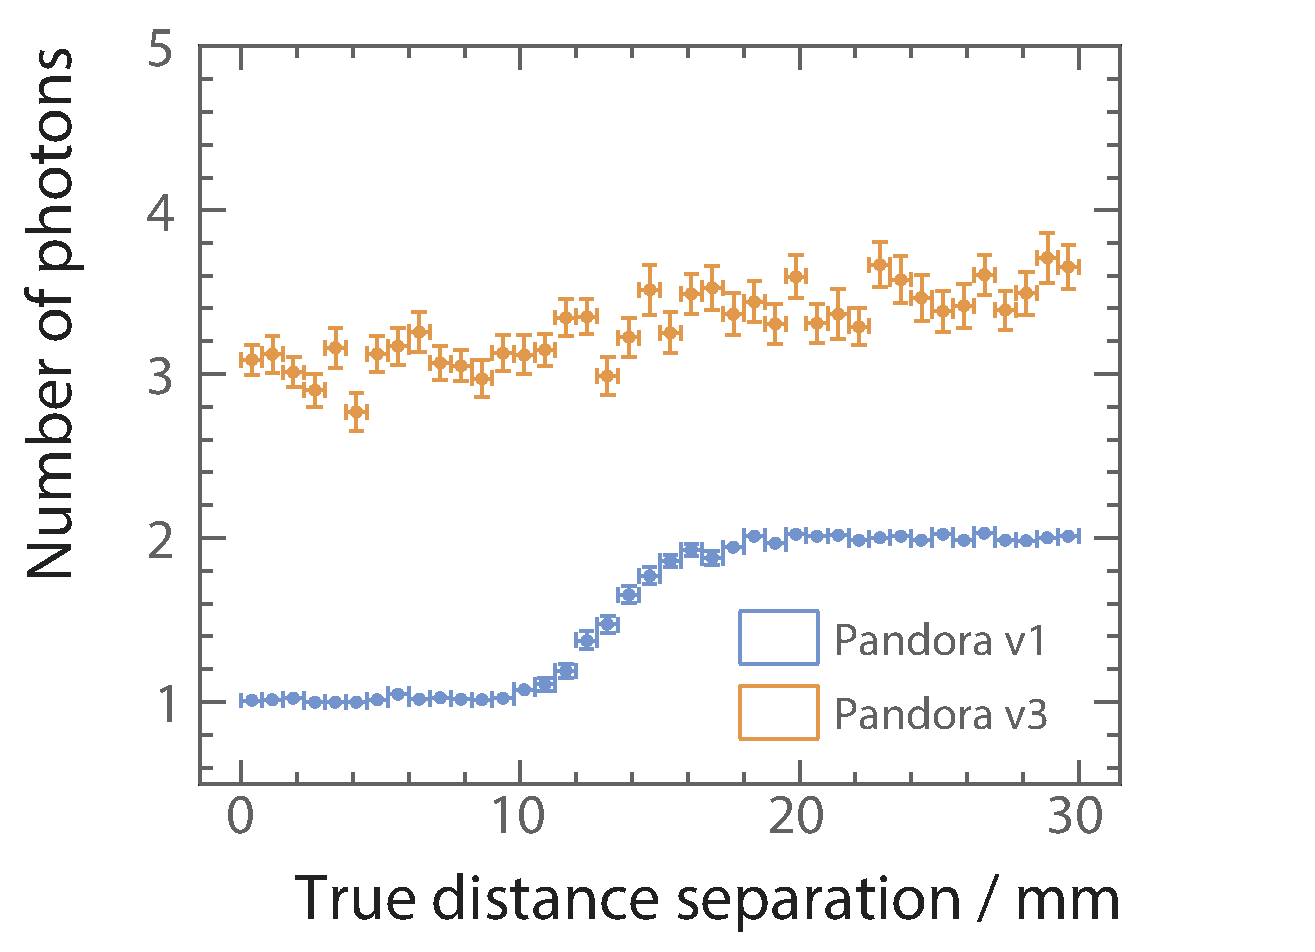
\includegraphics[width=\textwidth]{{photon/DoubleCompareN_p3.eps}}
        \caption{}
        \label{fig:photonDoubleCompareN_p}
    \end{subfigure}
    \begin{subfigure}[b]{0.45\textwidth}
        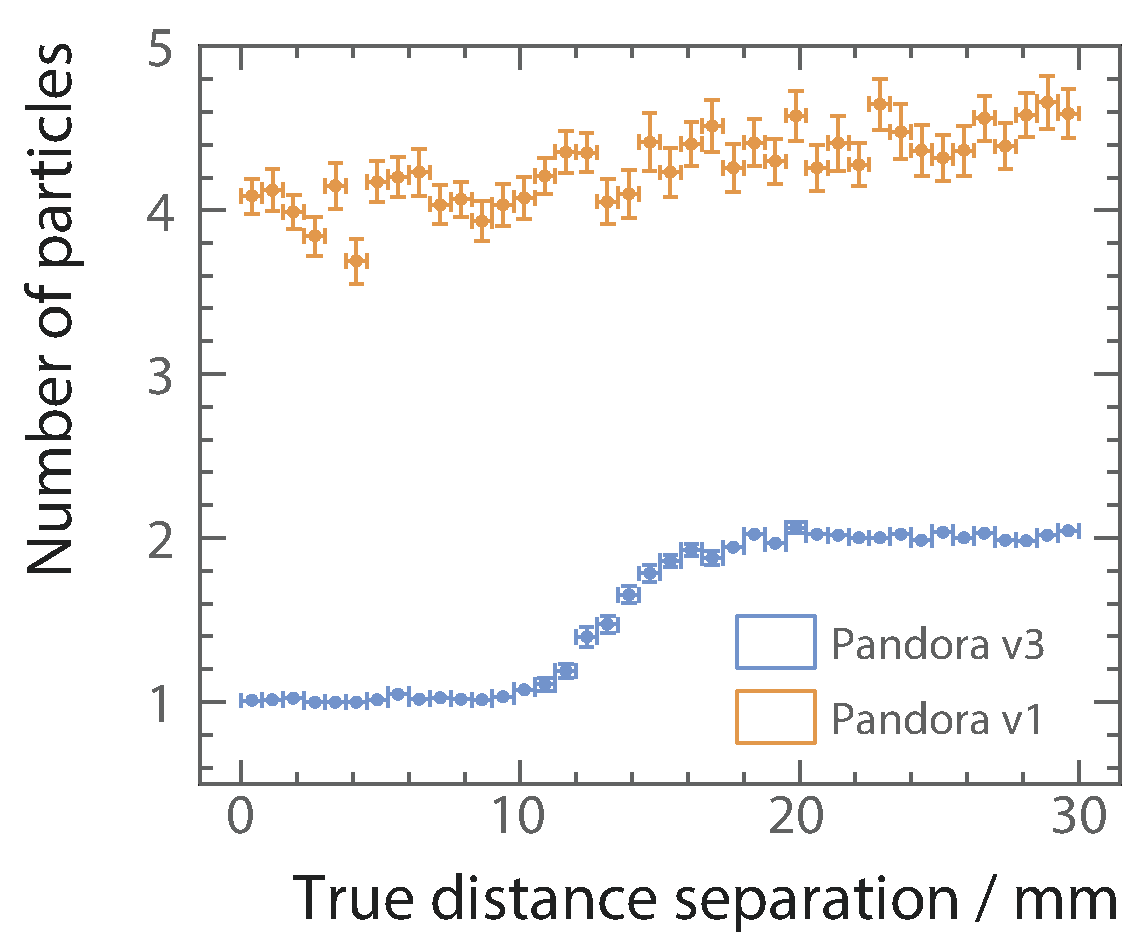
\includegraphics[width=\textwidth]{photon/DoubleCompareN_all3}
        \caption{}
        \label{fig:photonDoubleCompareN_all}
    \end{subfigure}
\caption[Average number of reconstructed photons and reconstructed particles, as a function of the MC distance separation.]
{Average numbers of reconstructed a) photons, and b) particles, as a function of the true distance separation between two photons, using  two-photon-per-event samples with photon energies of  500\,GeV and 50\,GeV. For both figures, the top orange and bottom blue dots represent the reconstruction with \pandora version 1 and version 3, respectively.}
\label{fig:photonDoubleCompareN}
\end{figure}

%The photon reconstruction is changed in \pandora version 2.



Another metric to reflect the improvement in photon reconstruction is the fraction of the fragment energy to the total energy in an event. In a two-photon-per-event sample, the fragment energy is defined as the total energy of particles excluding the two most energetic photons. Shown in \Figure{fig:photonDoubleFragEnergy}, using two-photon-per-event sample with photon energies of  500\,GeV and 50\,GeV, a reduction in fragment energy can be seen clearly going from \pandora version 1 to version 3. For the photon reconstruction in \pandora version 3, the average fragment energy fraction is below 0.1\% up to 30\,mm apart, whilst around 5\% energy would be in fragments for the reconstruction with \pandora version 1.
\begin{figure}[tbph]
\centering
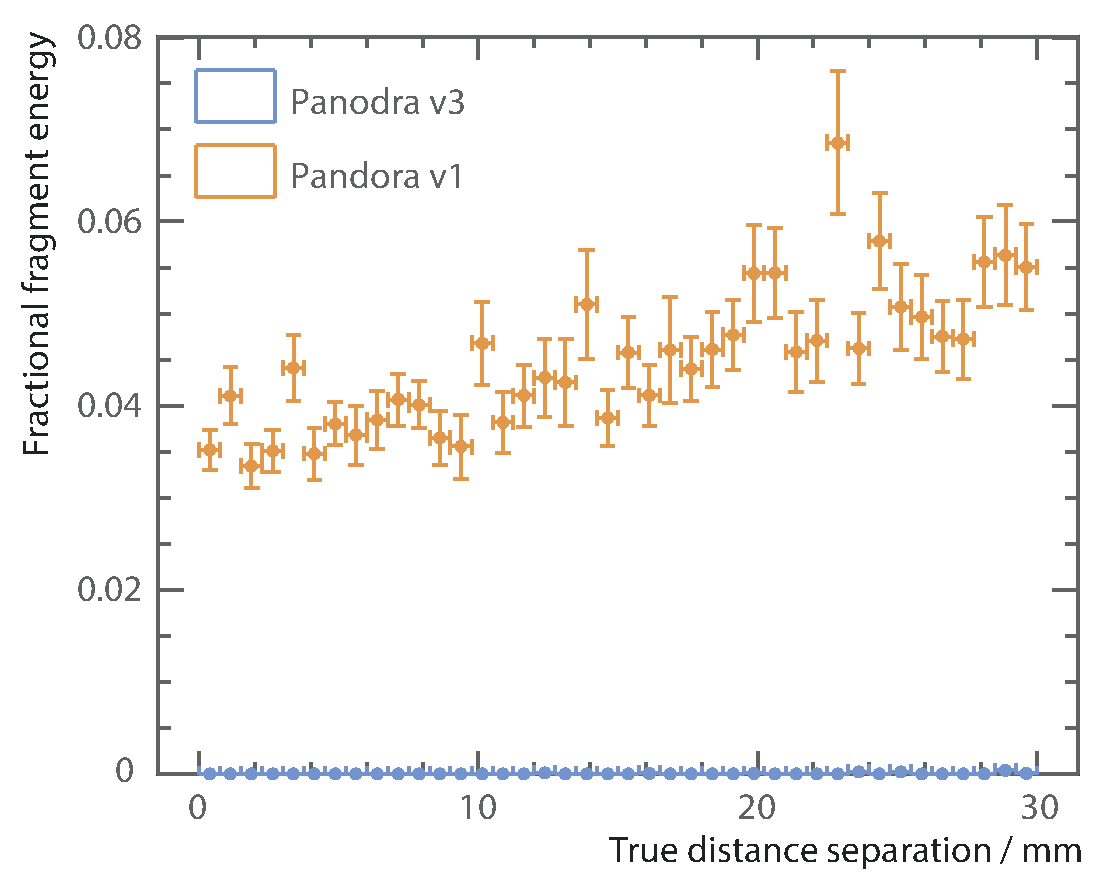
\includegraphics[width=0.85\textwidth]{photon/DoubleCompareFragEnergy3}
\caption[Average fraction fragments energy to the total energy, as a function of the MC distance separation]
{Average fraction of fragments energy to the total energy  in the event, as a function of the true distance separation between to photons, using a two-photon-per-event sample with photon energies of  500\,GeV and 50\,GeV. The top orange and bottom blue dots represent the reconstruction with \pandora version 1 and version 3 respectively. }
\label{fig:photonDoubleFragEnergy}
\end{figure}

%The photon reconstruction is changed in \pandora version 2.


The reduction in the fragments, as shown in the reconstruction of the single-photon-per-event and two-photon-per-event samples, leads to a small improvement in the jet energy resolution at a high jet energy. Using the same jet sample as in the previous section, the jet energy resolutions are better at total jet energies of 360 and 500\,GeV with the  photon reconstruction in \pandora version 3, as shown in \Figure{fig:photonJER}.

%This is due to more an aggressive photon reconstruction, which is more useful at a high-energy dense jet environment.



%The improvement of the photon is also demonstrated in \Chapter{chap:Tau}, where tau lepton decay modes are classified. Excellent photon reconstruction leads to a high classification rate.

\begin{figure}[tbph]
\centering
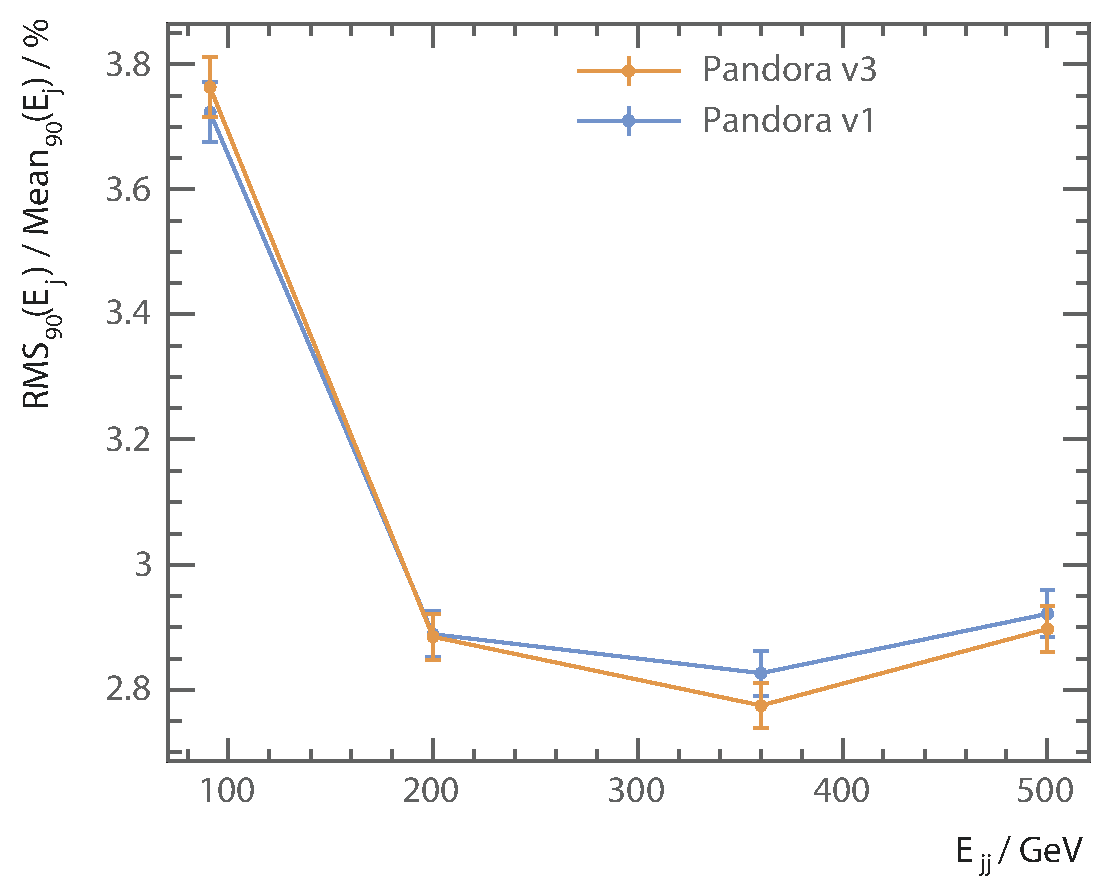
\includegraphics[width=0.85\textwidth]{photon/JERnew2}
\caption[Jet energy resolution as a function of the di-jet energy]
{Jet energy resolutions as a function of the total jet energy using \eeZuds, at barrel region. The top orange and bottom blue dots represent the  reconstruction with \pandora version 1 and version 3.}
\label{fig:photonJER}
\end{figure}


\subsection{Performance of individual photon algorithm}




%As stated before, the photon reconstruction algorithm in \Section{sec:photonRecostrcution} and the photon splitting algorithm in \Section{sec:photonSplitting}  improves the photon completeness and the photon pair resolution. The fragment removal algorithm in \Section{sec:photonFragRemoval} removes fragments in the \ECAL. High energy fragment removal algorithm in \Section{sec:photonHighEFragRemoval} removes fragments in the \HCAL.
Two-photon-per-event samples with photon energies of  500\,GeV and 500\,GeV is used to show the incremental improvement of the performance of individual photon algorithm, with different photon algorithms turned on and off. \FIGURE{fig:photonDoubleCompareAlgs} shows the average number of reconstructed particle as a function of true distance separation between two photons, reconstructed with full photon algorithms with \pandora version 3 (blue), reconstructed with only fragment removal algorithms in the \ECAL and photon reconstruction in  \pandora version 1 (orange), reconstructed with fragment removal algorithms in the \ECAL and the \HCAL and photon reconstruction in  \pandora version 1 (green), and reconstructed with \pandora version 1 (red).

%. Blue, orange, green, and red dots represent full photon reconstruction, reconstructed with only fragment removal algorithms in the \ECAL, reconstructed with fragment removal algorith%ms in the \ECAL and the \HCAL, and reconstructed with \pandora version 1, respectively.

%the average number of particle for a high energy photon pair, with photon energies of  500\,GeV and 500\,GeV, is shown in \Figure{fig:photonDoubleCompareAlgs}. Blue, orange, green, and red dots represent full photon reconstruction, reconstructed with only fragment removal algorithms in the \ECAL, reconstructed with fragment removal algorithms in the \ECAL and the \HCAL, and reconstructed with \pandora version 1, respectively.

For the reconstruction with fragment removal algorithm in the \ECAL (orange), the number of fragment is reduced significantly, when it is compared with photon reconstruction in \pandora version 1 (red). With the additional fragment removal algorithm in the \HCAL (green), the number of fragments is reduced further. At 40\,mm distance apart,  there is on average less than 0.05 fragment per photon pair for the reconstruction with fragment removal algorithms in the \ECAL and the \HCAL  (green).

The introduction of the photon reconstruction and photon splitting algorithm (blue) resolves the photon pair at a much shorter distance separation between two photons. Photon pairs start to be resolved at 5\,mm apart, and fully resolved at 15\,mm apart when reconstructed with full photon algorithms in \pandora version 3.
%, for a two-photon-per-event sample with photon energies of  500\,GeV and 500\,GeV,
%With previous photon reconstruction in \pandora version 1, the same photon pair starts to be resolved at 10\,mm apart and fully resolved at around 40\,mm apart.


\begin{figure}[tbph]
\centering
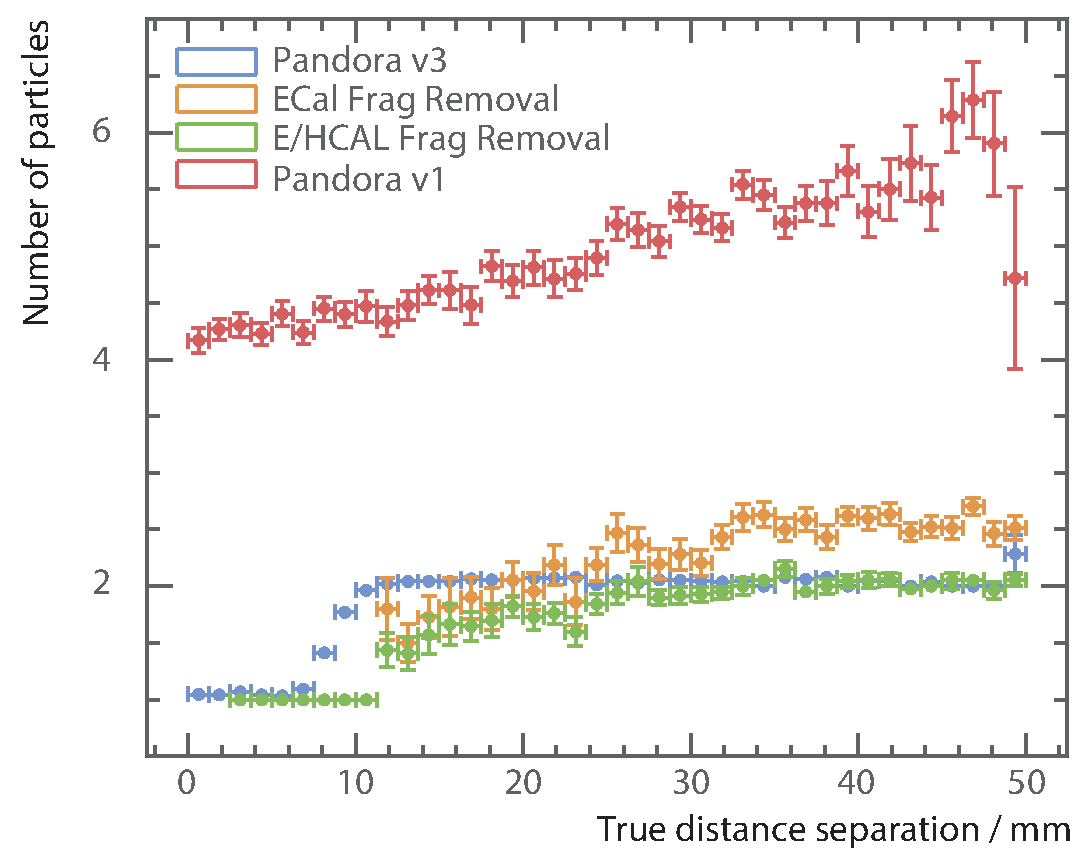
\includegraphics[width=0.85\textwidth]{photon/DoubleCompareAlg4}
\caption[Average number of photons, as a function of the MC distance separation for different algorithms combinations.]
{Average number of photons, as a function of the true distance separation between two photons, using a two-photon-per-event sample with photon energies of  500\,GeV and 500\,GeV. The blue, orange, green, and red dots represent the reconstruction with \pandora version 3, the reconstruction with fragment removal in the \ECAL and photon reconstruction in  \pandora version 1,  the reconstruction with fragment removal in the \ECAL and the \HCAL and photon reconstruction in  \pandora version 1, the reconstruction with \pandora version 1, respectively.}
\label{fig:photonDoubleCompareAlgs}
\end{figure}

\subsection{Photon reconstruction performance}

%In this section, the performance of the photon reconstruction as a function of photon energies will be described.
The photon reconstruction performance with \pandora version 3 is demonstrated with  single-photon-per-event and  two-photon-per-event samples.

\FIGURE{fig:photonSingleEffPerformance} shows the average single photon reconstruction  efficiency as a function of the true photon energies, using single-photon-per-event samples.  In single-photon-per-event samples, an event can have an efficiency of 1, or 0, depending on whether there is a reconstructed photon  corresponding to the true photon. The average single photon reconstruction efficiency is above 98\% for photons with energies above 2\GeV, and above 99.5\% for photons  with energies  above 100\,GeV.  The low efficiency in the first bin in \Figure{fig:photonSingleEffLow}, for photon energies in the range from 0 to 0.25\,GeV, is because photon reconstruction does not attempt to reconstruct photons with energies below 0.2\,GeV.

% is demonstrated in \Figure{fig:photonSingleEffPerformance}, using single-photon-per-event samples.

\begin{figure}[tbph]
\centering
    \begin{subfigure}[b]{0.45\textwidth}
        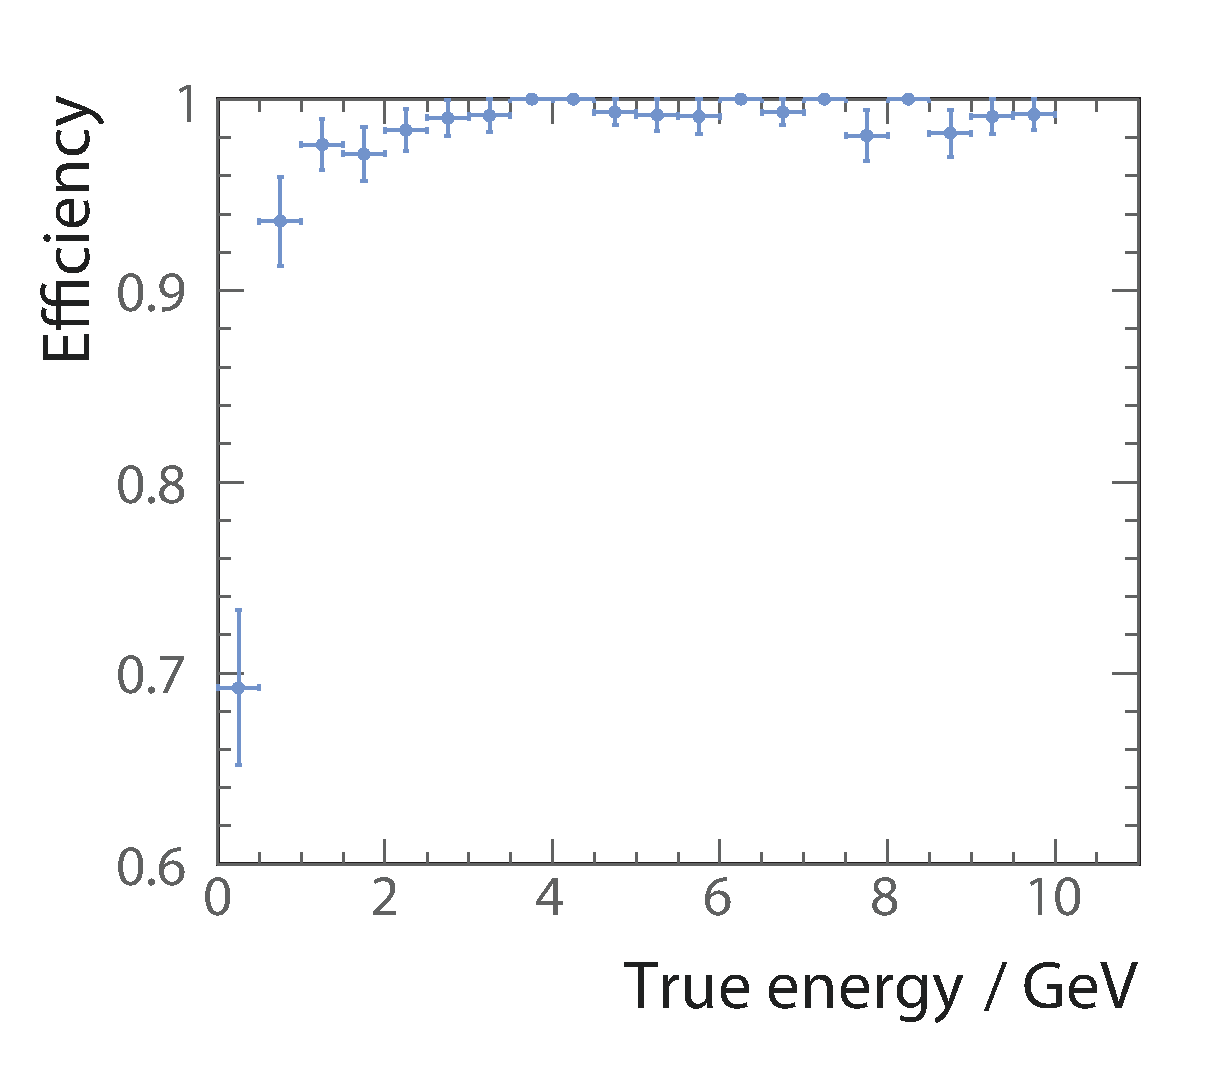
\includegraphics[width=\textwidth]{photon/singlePhotonEff3full}
        \caption{}
        \label{fig:photonSingleEffLow}
    \end{subfigure}
    \begin{subfigure}[b]{0.45\textwidth}
        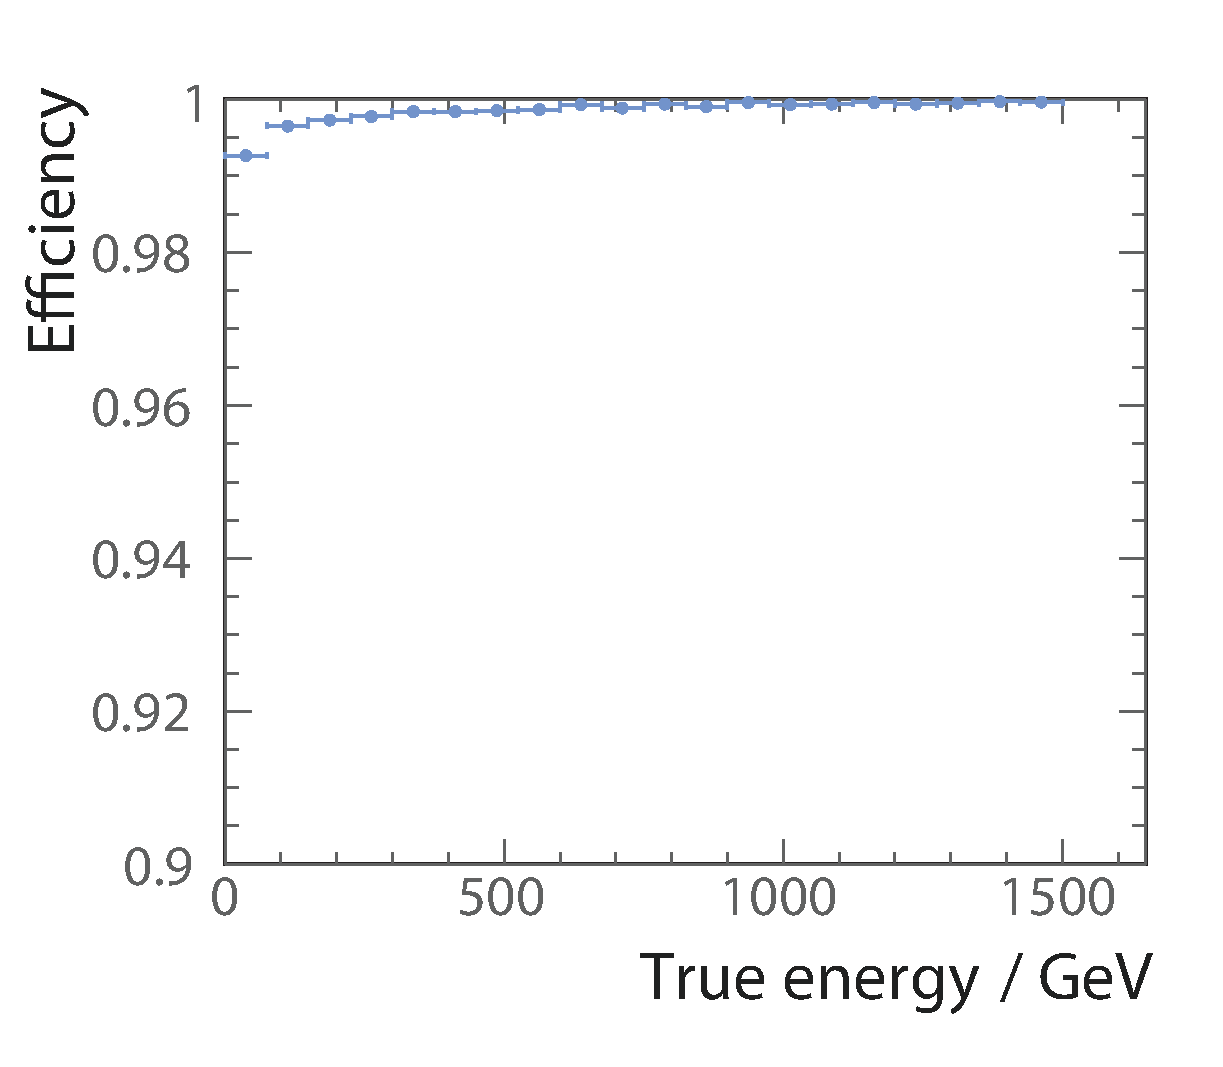
\includegraphics[width=\textwidth]{photon/singlePhotonEff2}
        \caption{}
        \label{fig:photonSingleEff}
    \end{subfigure}
\caption[Single photon reconstruction efficiency as a function of energy.]
{Single photon reconstruction efficiency as a function of true photon energies, using single-photon-per-event samples, for a) the low photon energy regime, and b) the high photon energy regime.}
\label{fig:photonSingleEffPerformance}
\end{figure}

\FIGURE{fig:photonDoubleCompareN_pN_all} shows  the average numbers of reconstructed photons and particles  as a function of the true distance separation between two photons, using a two-photon-per-event sample with photon energies of  500\,GeV and 500\,GeV. A good match between the number of photons and the number of particles is achieved. The average numbers of photons and particles are  both fewer than 2.05 for a distance separation beyond 20\,mm, less that 1 fragment produced per 20 events.


%For  two-photon-per-event samples, there are very few fragments.

\begin{figure}[tbph]
\centering
        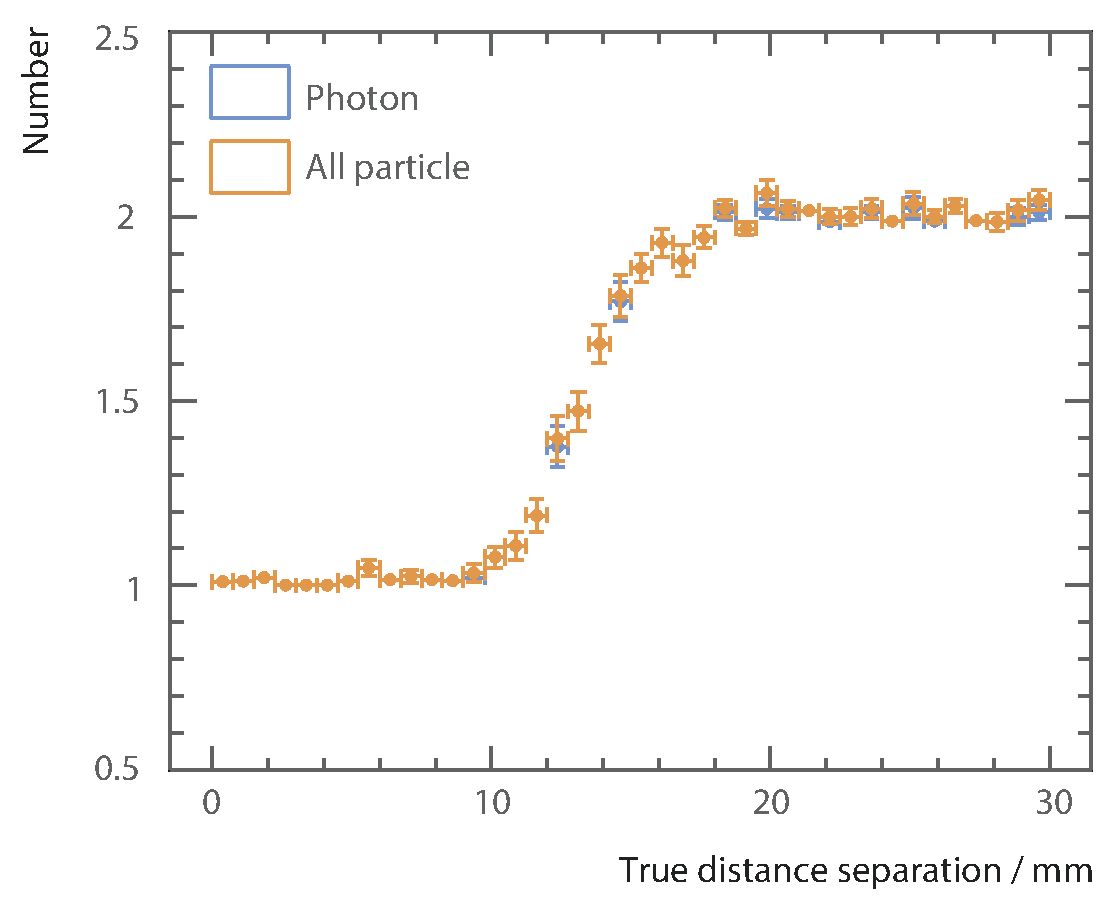
\includegraphics[width=0.85\textwidth]{photon/DoubleN_pN_all2}
        \caption{Average numbers of reconstructed photon  (blue) and particle (orange), as a function of the true distance separation between two photons, using two photons of 500\,GeV and 50\,GeV per event samples. }
        \label{fig:photonDoubleCompareN_pN_all}
\end{figure}

The ability to  resolve of a photon pair depends on energies of two photons. \FIGURE{fig:photonDoubleCompareEnergies} shows the average number of photon reconstructed using two-photon-per-event samples as a function of the true distance separation between two photons, for different photon energies. When the energies of two photons are similar, the distance of two photons starting to be resolved is shorter. This is because that when the two photon showers have similar sizes, the \peakFinding algorithm can exploit the symmetry in the size of the EM showers. For example, 500\,GeV$-$500\,GeV photon pair and 10\,GeV$-$10\,GeV photon pair start to be resolved at 6\,mm apart, which is about one \ECAL cell length in the simulated nominal \ILD detector. In contrast, photon pairs with different energies, for example 500\,GeV$-$50\,GeV and  100\,GeV$-$10\,GeV pairs, start to be resolved at 10\,mm apart, which is about two \ECAL cells length.

For an energetic photon, it is easier to identify the photon, because the electromagnetic shower core is denser and contains more energies than the peripheral calorimeter hits. Therefore separating two energetic photons is easier than separating two low-energy photons. As shown in \Figure{fig:photonDoubleCompareEnergies}, at 20\,mm distance apart, 500\,GeV$-$500\,GeV photon pairs are fully resolved, whereas approximately only 60\% of 10\,GeV$-$10\,GeV photon pairs are resolved.

\begin{figure}[tbph]
\centering
        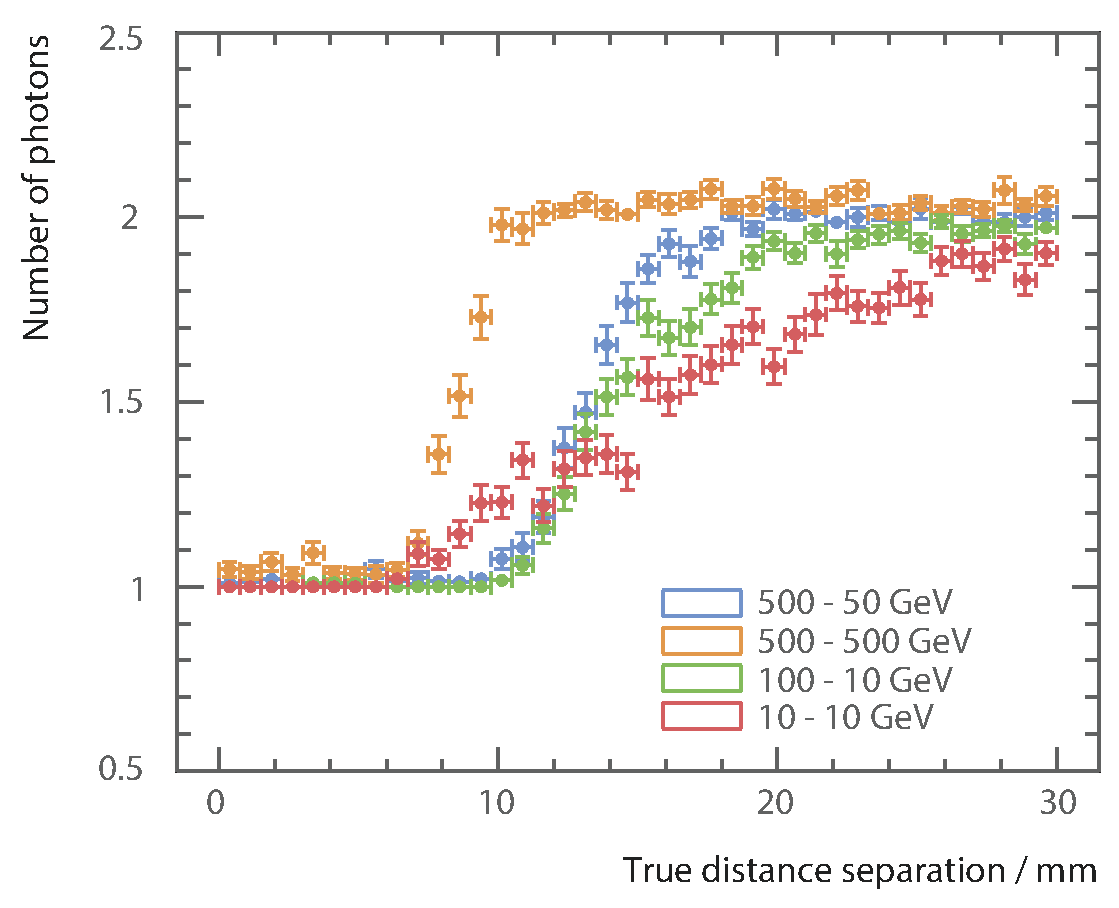
\includegraphics[width=0.85\textwidth]{photon/DoubleCompareEnergies2}
        \caption{Average numbers of reconstructed photon for four different photon pairs: 500\,GeV$-$50\,GeV (blue), 500\,GeV$-$500\,GeV (orange), 100\,GeV$-$10\,GeV (green), and 10\,GeV$-$10\,GeV (red), as a function of the true distance separation between two photons.}
        \label{fig:photonDoubleCompareEnergies}
\end{figure}

